


\documentclass[aps,pre,superscriptaddress]{article}

\usepackage{xcolor}
\usepackage{preamble}
\usepackage{color}
\usepackage{verbatim}
\usepackage{graphicx}
\usepackage{url}
\graphicspath{ {./figures} }

\begin{document}

% \begin{abstract}
% \end{abstract}

\title{SBM-WCC Ian's Document}
\author{Ian Chen and others}
%\noaffiliation
\date{\today}
\maketitle

\section{Introduction}
See the preprint~\cite{Park25-02}.

\section{Materials and Methods}

We used 122 networks --- 120 networks from the Netzschleuder network catalogue~\cite{Netzschleuder} and two other networks from ~\cite{Park24-11}.
The networks range in size, from 11 to 13,989,436 nodes, and 13 to 117,185,083 edges.

We used graph-tool~\cite{graph-tool} to optimize for minimum description length (MDL) of the degree-corrected flat and nested models.

\section{Nested-SBM on Empirical Networks}

\begin{figure}
	\centering
	\begin{subfloat}
		\centering
		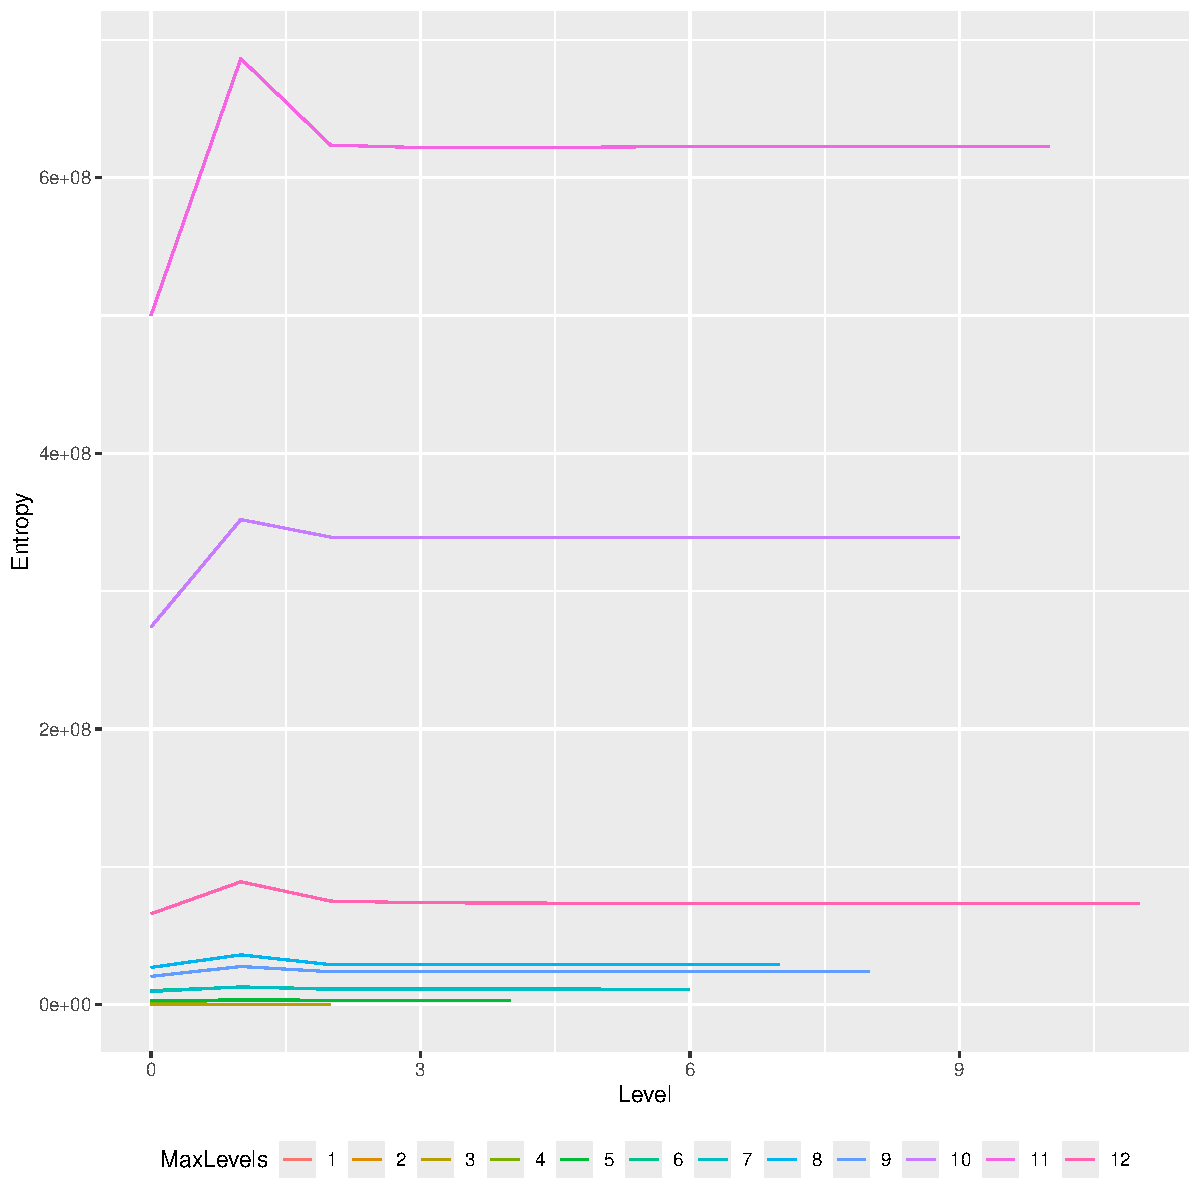
\includegraphics[width=0.48\textwidth]{fig1.pdf}
	\end{subfloat}
	\begin{subfloat}
		\centering
		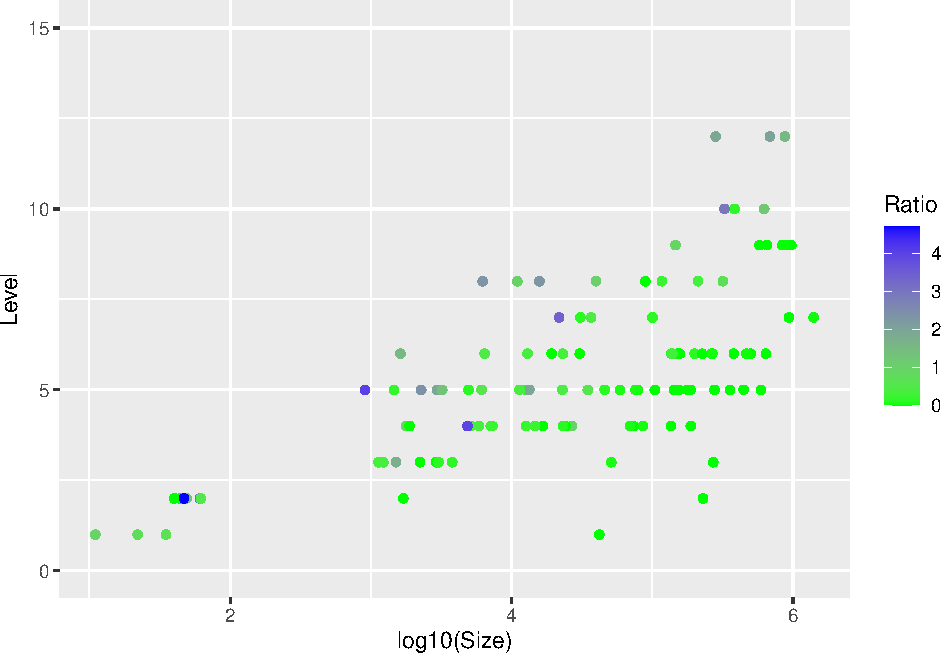
\includegraphics[width=0.48\textwidth]{fig2.pdf}
	\end{subfloat}
	\caption{Entropy and Clusters across Hierarchical-SBM Levels:
		On all empirical networks (120).
		For each plot, we take the mean across all networks with MaxLevels number of inferred levels.
		Left: The description length is calculated according to the Degree Corrected (non-nested) SBM model.
		Right: The number of clusters (log scale).
	}
	\label{figs:fig1}
\end{figure}

\begin{figure}[ht]
	\centering
	\begin{subfloat}
		\centering
		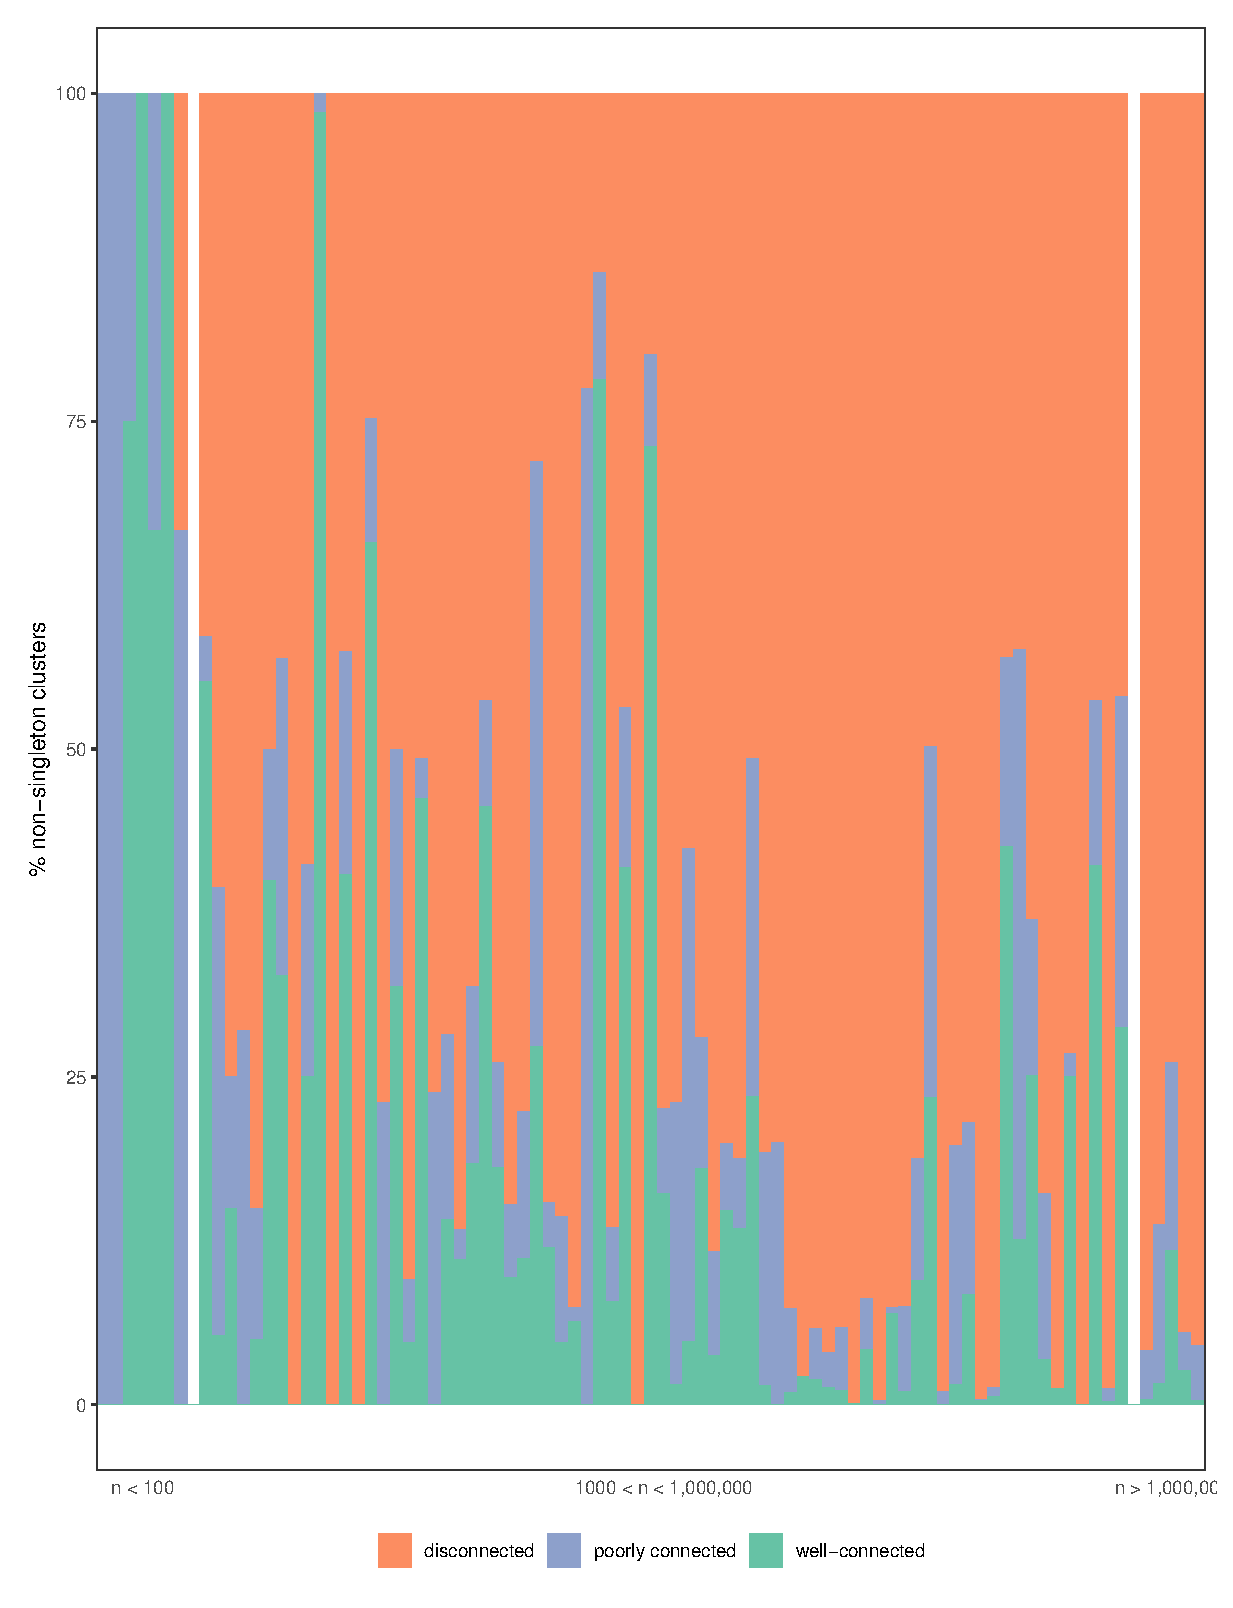
\includegraphics[width=\textwidth]{nested_sbm_conn.eps}
	\end{subfloat}
	% \begin{subfloat}
	% 	\centering
	% 	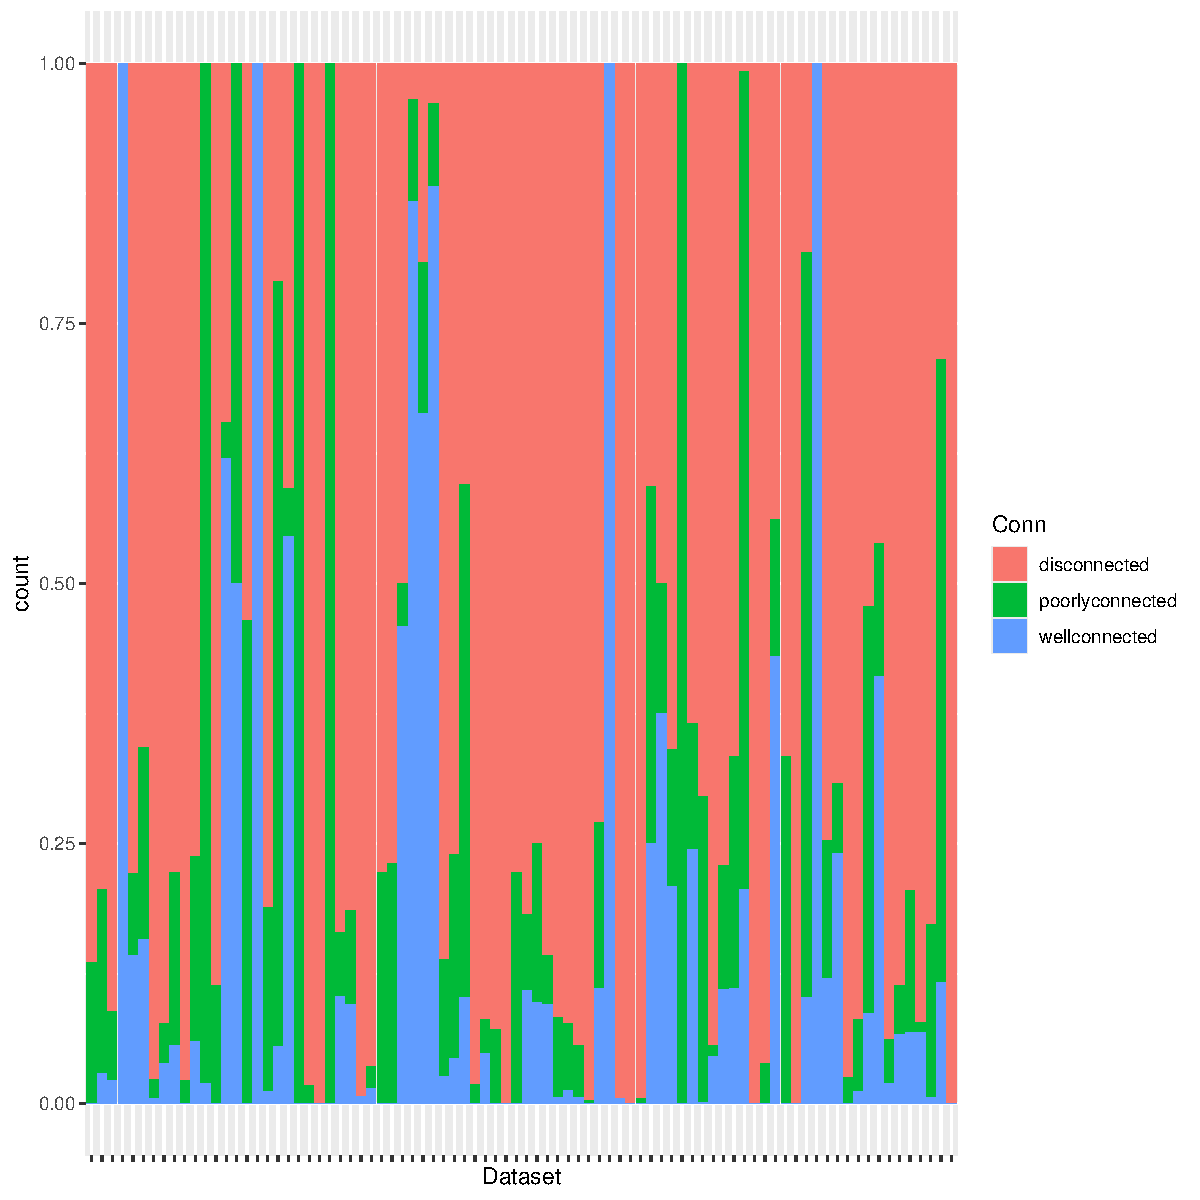
\includegraphics[width=0.8\textwidth]{fig3c.pdf}
	% \end{subfloat}
	\caption{
		Connectivity of Hierarchical-SBM Clusters.
		On the non-bipartite empirical networks (85).
		Each bar is a network, sorted in increasing network size.
		The y-axis shows percentage disconnected, poorly connected, and well-connected
	}
	\label{figs:nested_sbm_conn}
\end{figure}

\begin{figure}[ht]
	\centering
	\begin{subfloat}
		\centering
		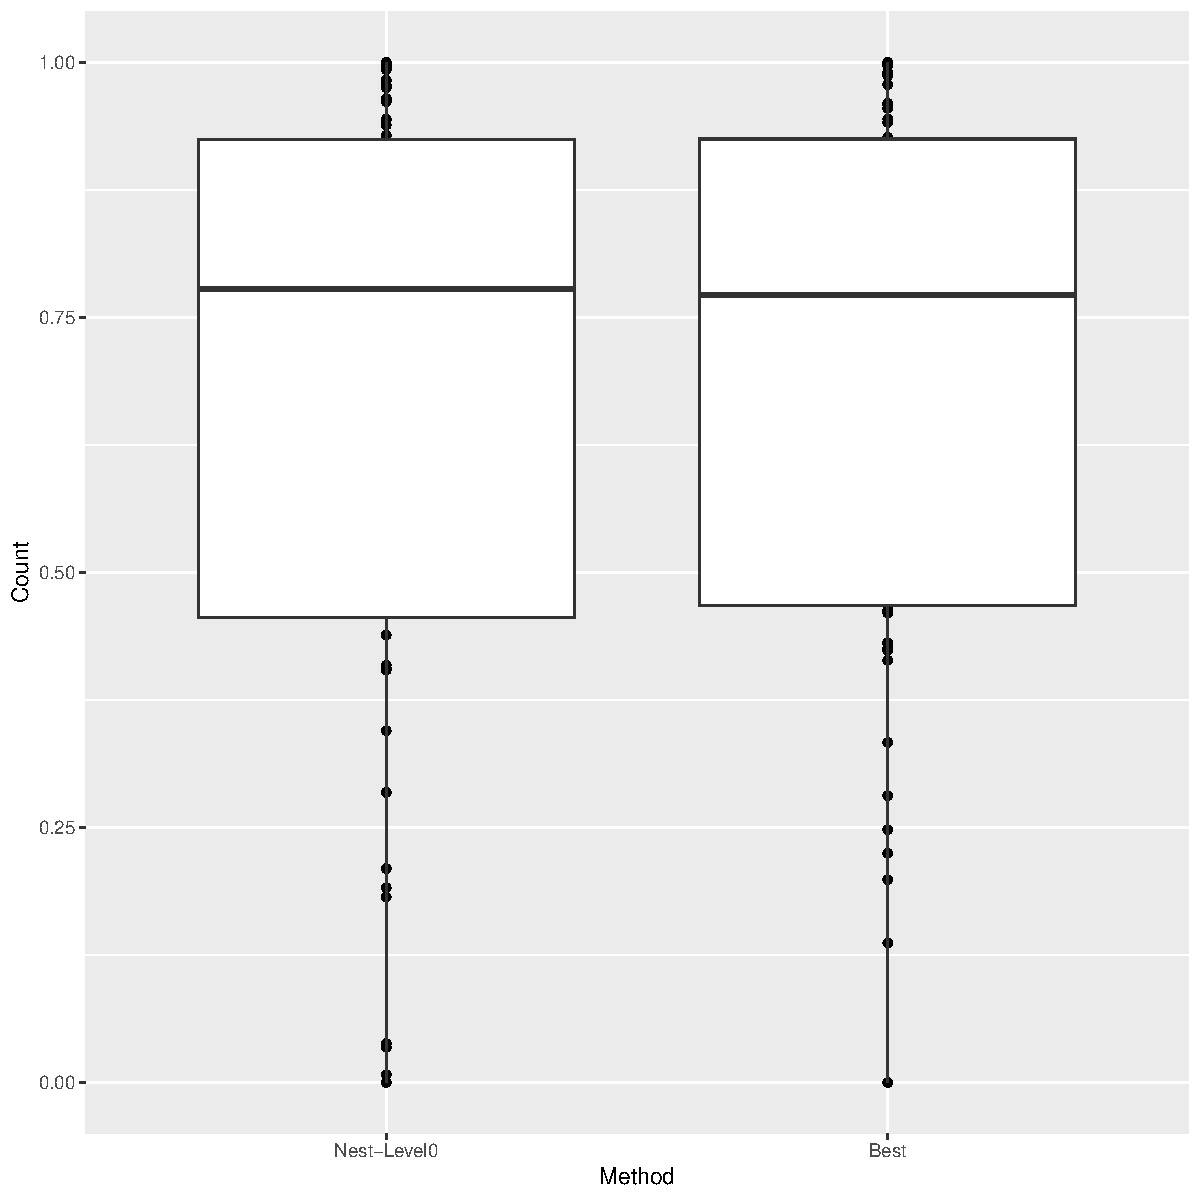
\includegraphics[width=0.4\textwidth]{fig4a.pdf}
	\end{subfloat}
	\begin{subfloat}
		\centering
		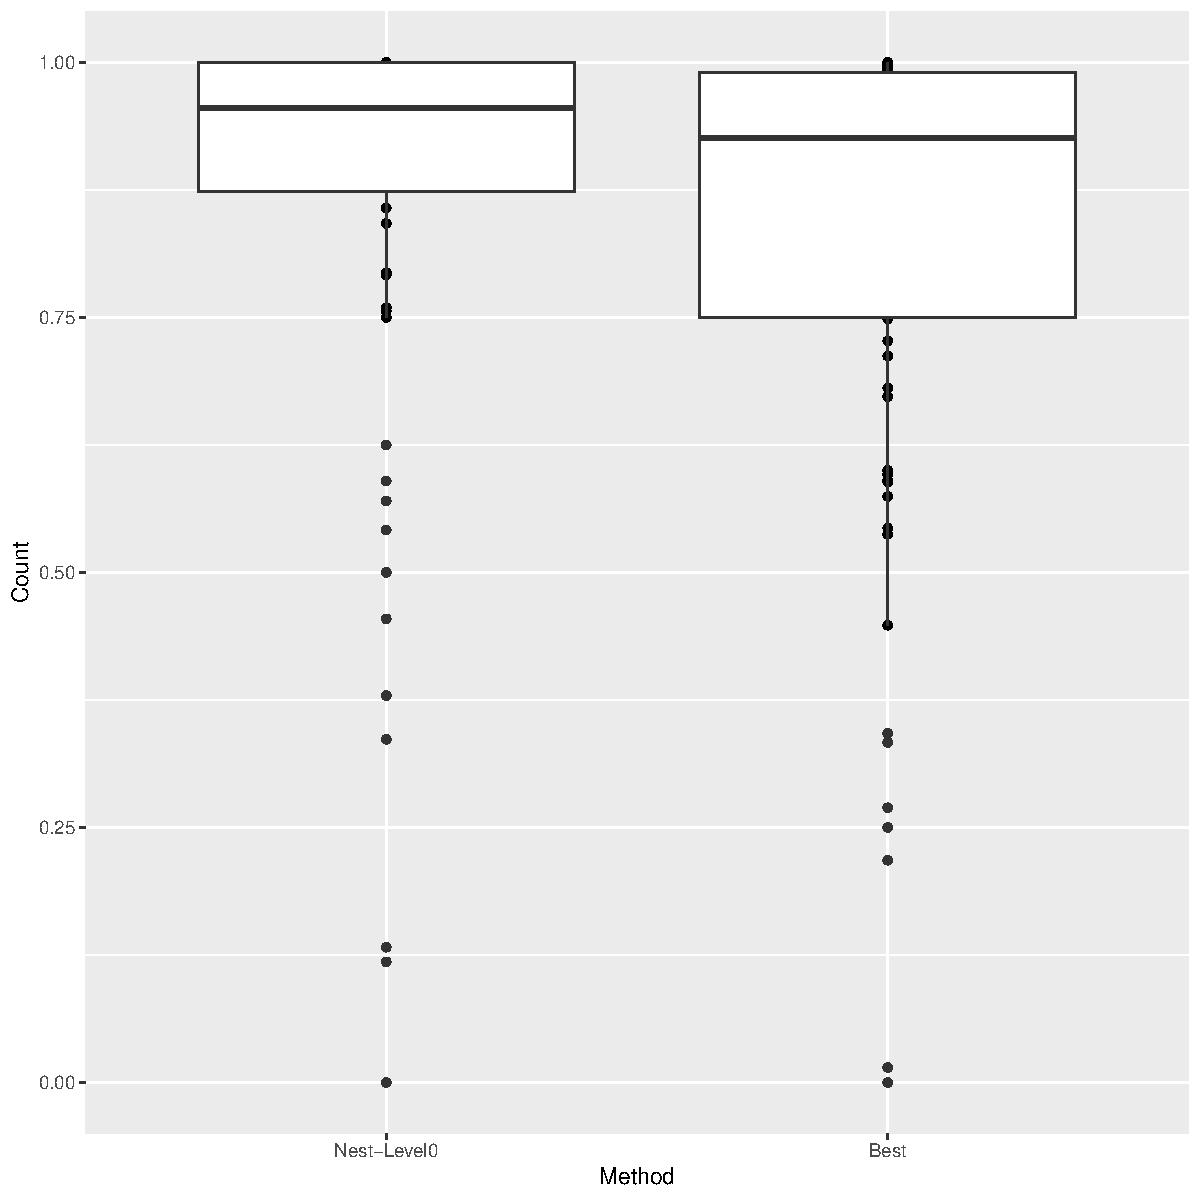
\includegraphics[width=0.4\textwidth]{fig4b.pdf}
	\end{subfloat}
	\caption{Connectivity Comparison:
		On the non-bipartite empirical networks (85).
		The x-axis indicates the method.
		Left: Proportion of clusters that are disconnected.
		Right: Proportion of clusters that are poorly-connected (including disconnected).
	}
	\label{figs:fig3}
\end{figure}

On average, the best layer by itself (via description length) is Layer 0 (Figure \ref{figs:fig1}).
Moreover, on all the 120 empirical networks (except for petster), the layer with the lowest description length (compared to the other layers) is Layer 0 --- on petster, it was layer 4 (out of 10 layers).

We conducted paired t-tests to test whether there are differences in the connectivity between nested and flat degree-corrected SBM models.
Where is no statistical difference between the percentage of disconnected clusters (p = 0.5264), but there was a difference in the well-connected proportions (p = 0.0193), with flat having better connectivity.

\section{Other SBMs}

Here, we give a brief overview of other SBM models and inference algorithms, and investigate their runtime and connectivity.
See ~\cite{funke19-04} for a more in-depth discussion of the variants that does not mention connectivity nor runtime.

\subsection{Models}

The main variants of SBM are the degree corrected and non-degree corrected SBM models for flat and also hierarchical.
Here, we use the microcanonical formulation~\cite{peixoto17-01}~\cite{peixoto14-03}.
In addition, closed formulas have been derived that speed up the calculation of the likelihood function by including the number of blocks~\cite{come15-12}.
Finally, there are SBM models that specialize on disassociative structures in bipartite graphs~\cite{yen20-09}.
Since this is a subclass of the other models, here we do not investigate it further.

We follow the naming convention in ~\cite{funke19-04}.
See the formulas in \ref{sbm-formulas}.

\subsection{Inference Algorithms}

Inferring the number of blocks and optimizing the partition given a number of blocks is difficult to do exactly.
Above, we investigated Peixoto's Agglomerative Heuristic~\cite{peixoto14-01}, which starts with a set of singleton clusters and merges them.
In addition, there is the Kernighan-Lin algorithm~\cite{kernighan70-02} which starts with a random partition and does a local search through node moves.

TODO: something about dcd

\clearpage
\subsection{Results on PySBM}

Datasets (10 smallest in the medium list, by node count -- 906 to 2115 nodes):
empirical:
\begin{verbatim}
dnc,uni_email,polblogs,faa_routes,netscience,new_zealand_collab
,collins_yeast,interactome_stelzl,bible_nouns,at_migrations    
\end{verbatim}

\begin{figure}[!htpb]
	\centering
	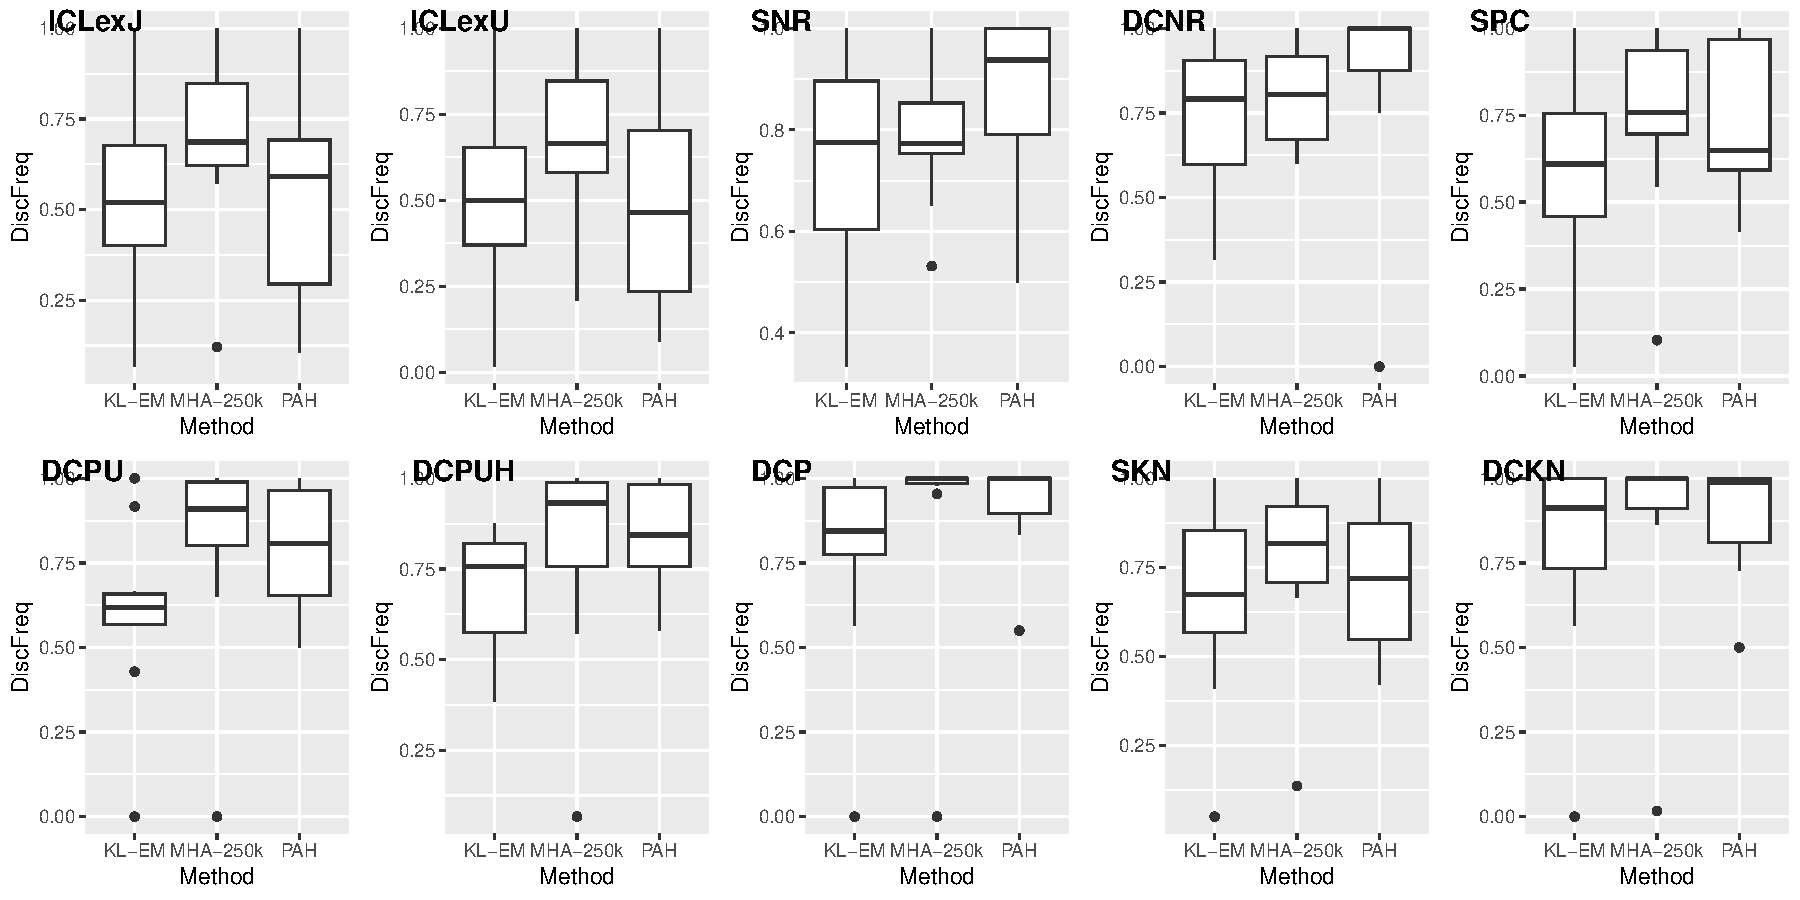
\includegraphics[width=\textwidth]{figures/pysbm_disc.pdf}
	\caption[]{
		\textbf{Connectivity of PySBM on medium empirical non-bipartite networks}
		Each subfigure shows the connectivity of three PySBM inference algorithms on each (non-nested) SBM variant.
		The nested versions are ommitted because PySBM only HPAH can run on a nested partition.
		For all models besides SCP, DCPU, and DCPUH (where we used the blocks in graph-tool), we used the same number of blocks for PySBM as in chosen-SBM.
		We used the 10 smallest datasets in the medium empriical datasets, from 906 to 2115 nodes.
		DiscFrequency is the proportion of non-singleton clusters that are disconnected.
	}
	\label{fig:pysbm_disc.pdf}
\end{figure}

\begin{figure}[!htpb]
	\centering
	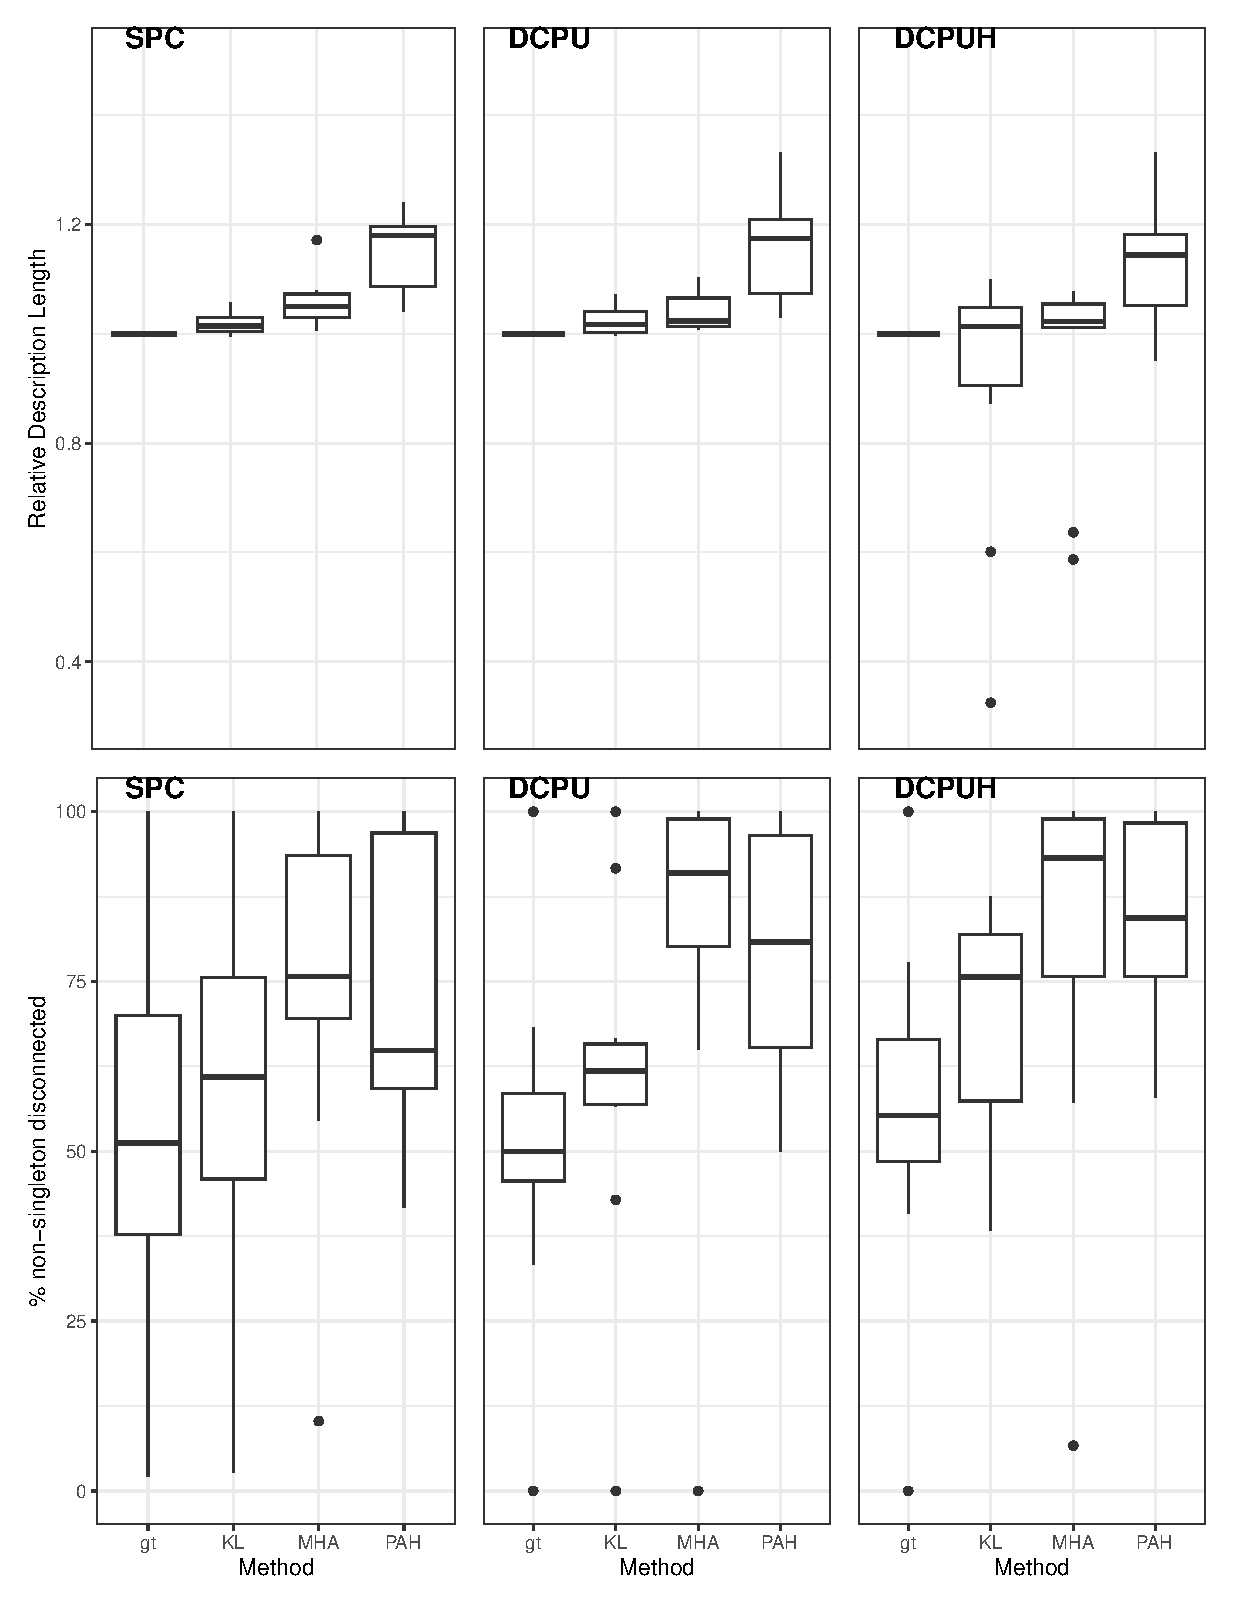
\includegraphics[width=\textwidth]{figures/pysbm_v_graph_tool_flat.eps}
	% 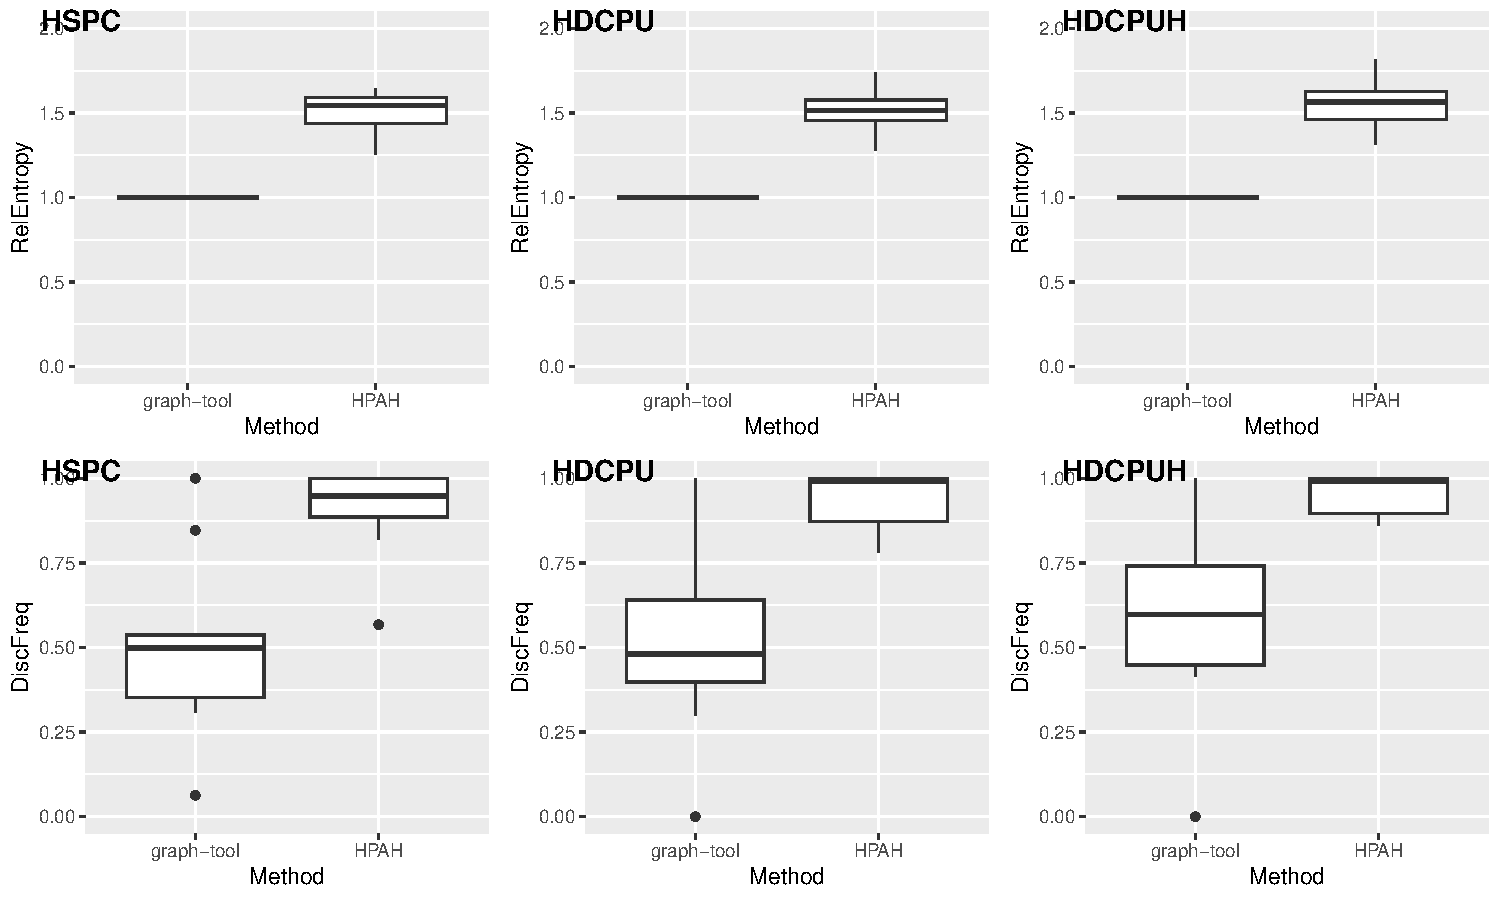
\includegraphics[width=0.9\textwidth]{figures/pysbm_v_graph_tool_nested.pdf}
	\caption[]{
		\textbf{Comparison of PySBM against graph-tool on medium empirical non-bipartite networks}
		The first two rows compare the entropy and disconnected frequencies on non-nested models.%, and the next two rows compare on nested models.
		We used the same number of blocks for PySBM as in graph-tool.% (but not the number of layers in the nested case).
		We calculate the description length according to each model and report RelEntropy normalized with dividing by graph-tool's clustering.
		DiscFrequency is the proportion of non-singleton clusters that are disconnected.
		We see that a worse description length is consistent with more disconnected clusters.
	}
	\label{fig:comparison_flat.pdf}
\end{figure}

\clearpage
\section{Results on Synthetic Networks}

\begin{figure}[!htpb]
	\centering
	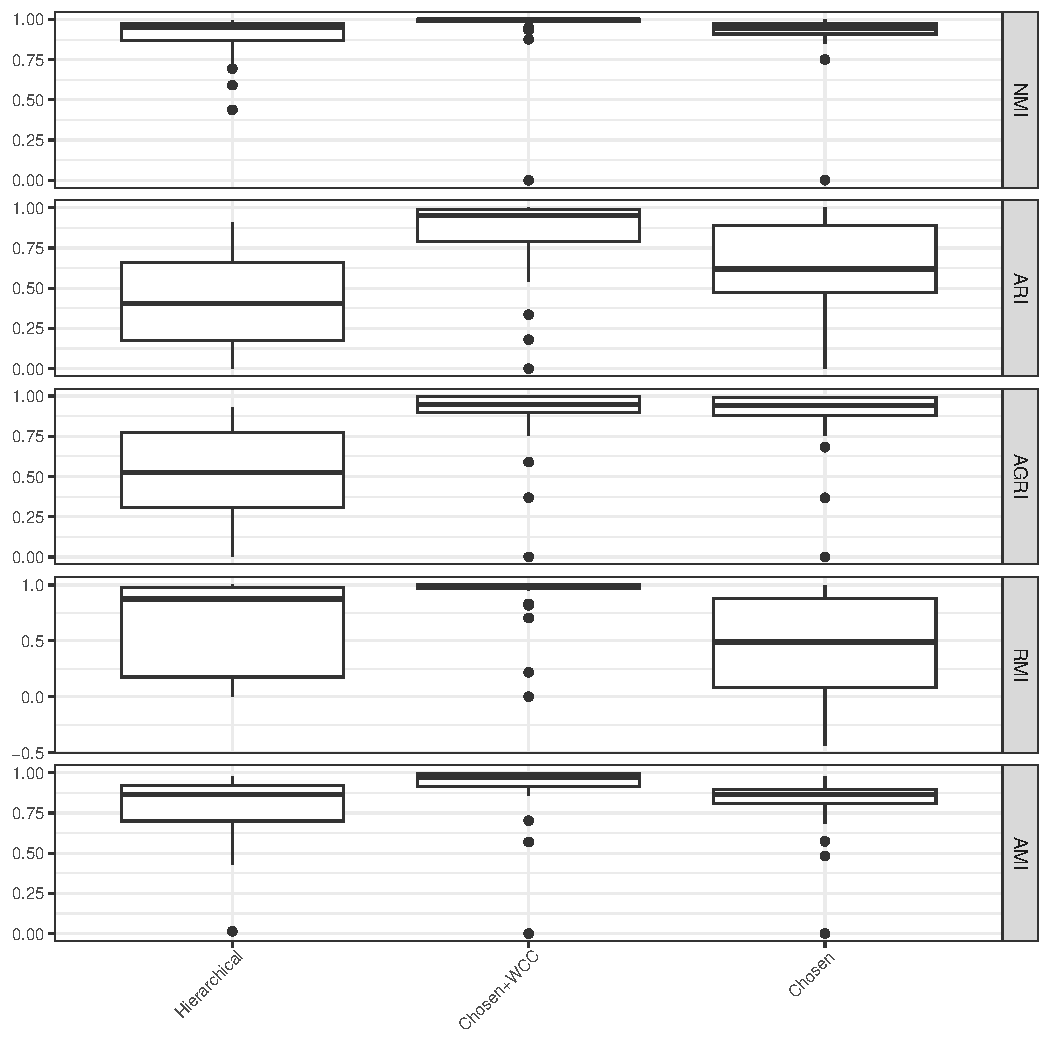
\includegraphics[width=0.9\textwidth]{figures/accuracy_box.pdf}
	\caption[]{\textbf{Clustering accuracy on LFR and RECCS synthetic networks}  Each subfigure shows the results on five different clustering accuracy metrics (NMI, ARI, AGRI, RMI, and AMI). The biggest differences in accuracies come from ARI, AGRI, and RMI, where chosen SBM + WCC has the best accuracy followed by chosen SBM and then hierarchical SBM. On NMI and AMI, although there may be a slight advantage to using chosen SBM + WCC, the accuracy differences across the different methods were small. Notes: SBM+WCC timeout on cit\_patents-0.5(LFR), SBM+WCC oom on wiki\_topcats-0.01(RECCS), and nested SBM oom on oc-0.001(LFR). Data only shown for those datasets where all methods completed successfully. Total of 27 networks.}
	\label{fig:synthetic-accuracy}
\end{figure}

\begin{figure}[!htpb]
	\centering
	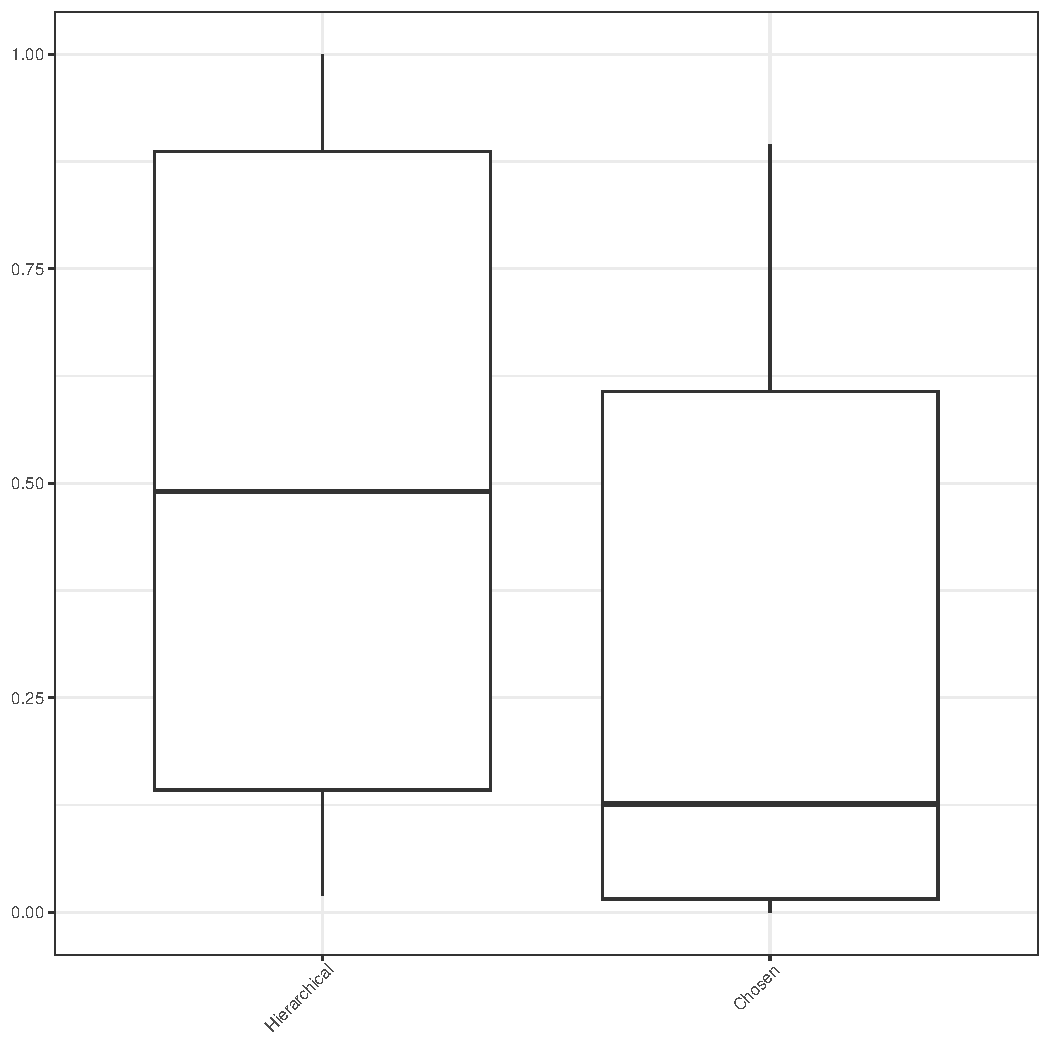
\includegraphics[width=0.9\textwidth]{figures/conn_box.pdf}
	\caption[]{\textbf{Proportion of disconnected clusters produced by Hierarchical SBM and Chosen SBM on synthetic LFR and RECCS networks}  We see that hierarchical SBM tends to produce clusterings with higher proportions of disconnectd clusters than chosen SBM on these synthetic networks. Notes: SBM+WCC timeout on cit\_patents-0.5(LFR), SBM+WCC oom on wiki\_topcats-0.01(RECCS), and nested SBM oom on oc-0.001(LFR). Data only shown for those datasets where all methods completed successfully. Total of 27 synthetic networks.}
	\label{fig:synthetic-connectivity}
\end{figure}
%Minhyuk: write down how many networks 

\begin{figure}[!htpb]
	\centering
	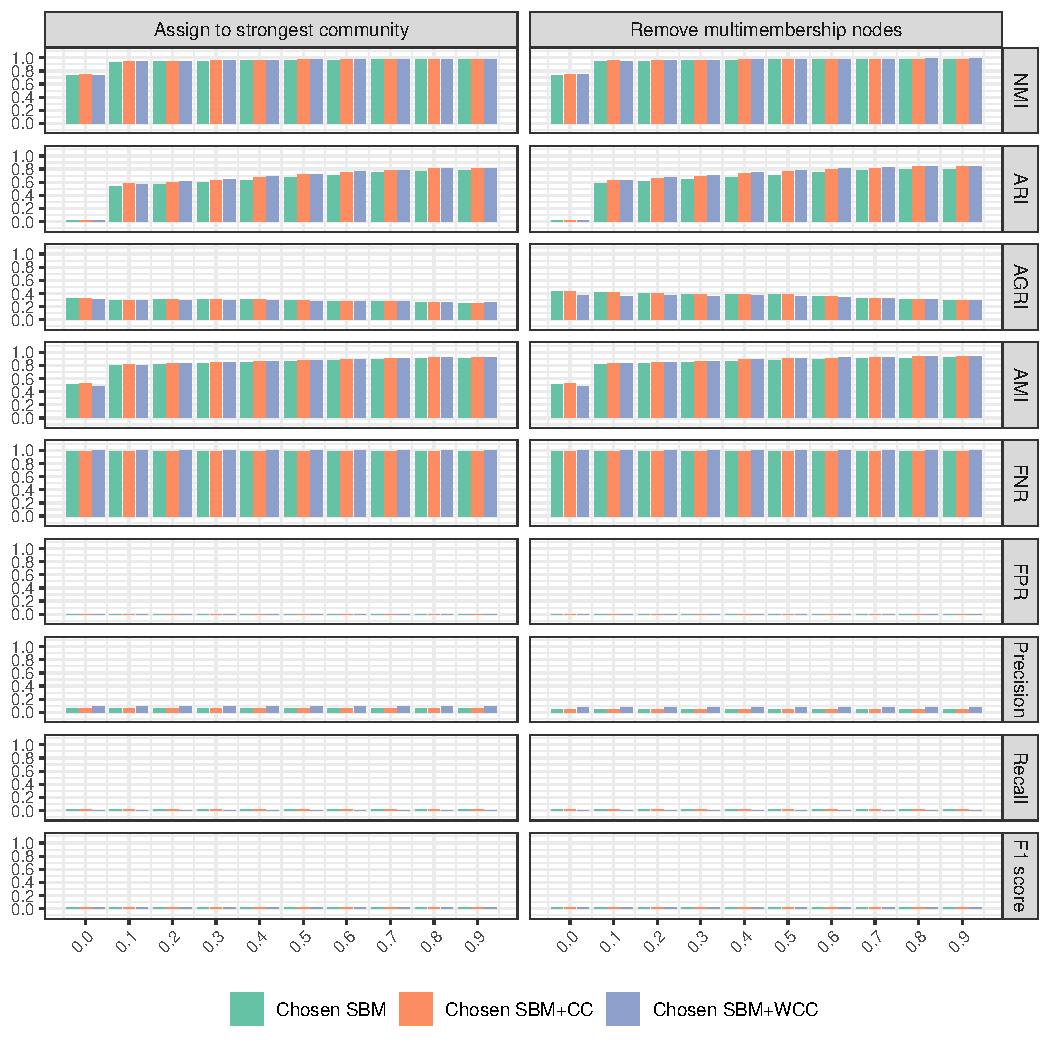
\includegraphics[width=0.9\textwidth]{figures/density_dblp_accuracy.pdf}
	\caption[]{\textbf{Various Clustering Accuracies for Varying Density Levels on the DBLP SNAP real-world network with ground-truth}}
	\label{fig:density-dblp-accuracy}
\end{figure}

\begin{figure}[!htpb]
	\centering
	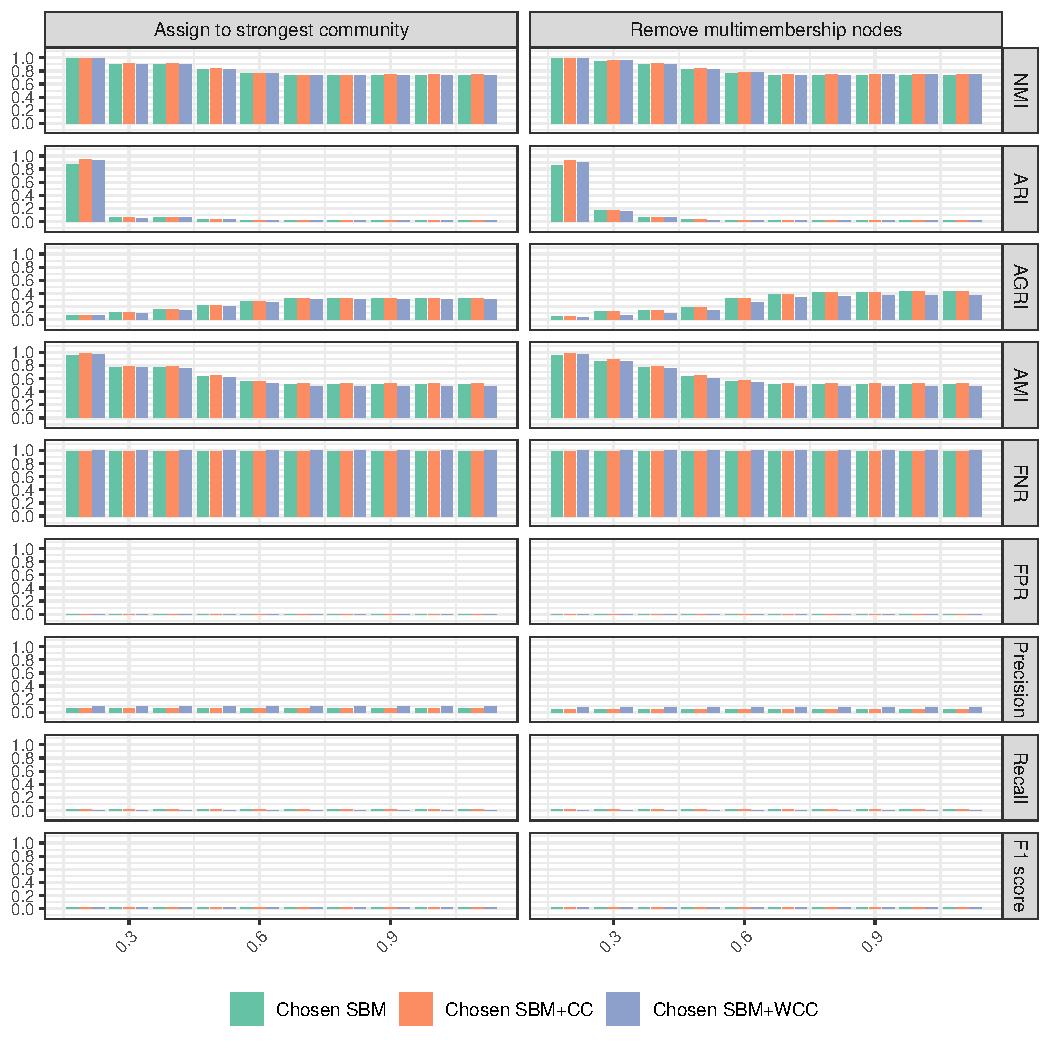
\includegraphics[width=0.9\textwidth]{figures/noise_dblp_accuracy.pdf}
	\caption[]{\textbf{Various Clustering Accuracies for Varying Noise Levels on the DBLP SNAP real-world network with ground-truth}}
	\label{fig:noise-dblp-accuracy}
\end{figure}

\begin{figure}[!htpb]
	\centering
	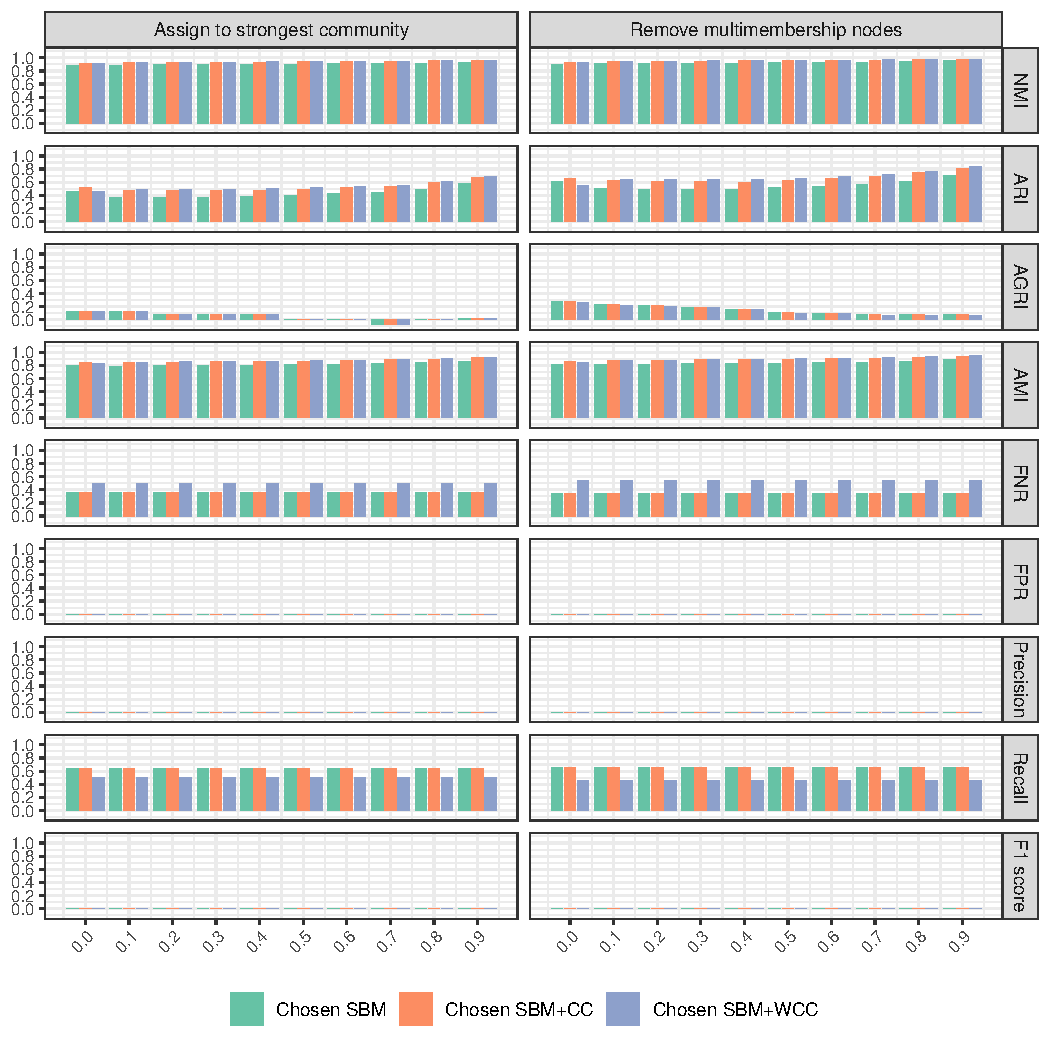
\includegraphics[width=0.9\textwidth]{figures/density_livejournal_accuracy.pdf}
	\caption[]{\textbf{Various Clustering Accuracies for Varying Density Levels on the Livejournal SNAP real-world network with ground-truth}}
	\label{fig:density-livejournal-accuracy}
\end{figure}

\begin{figure}[!htpb]
	\centering
	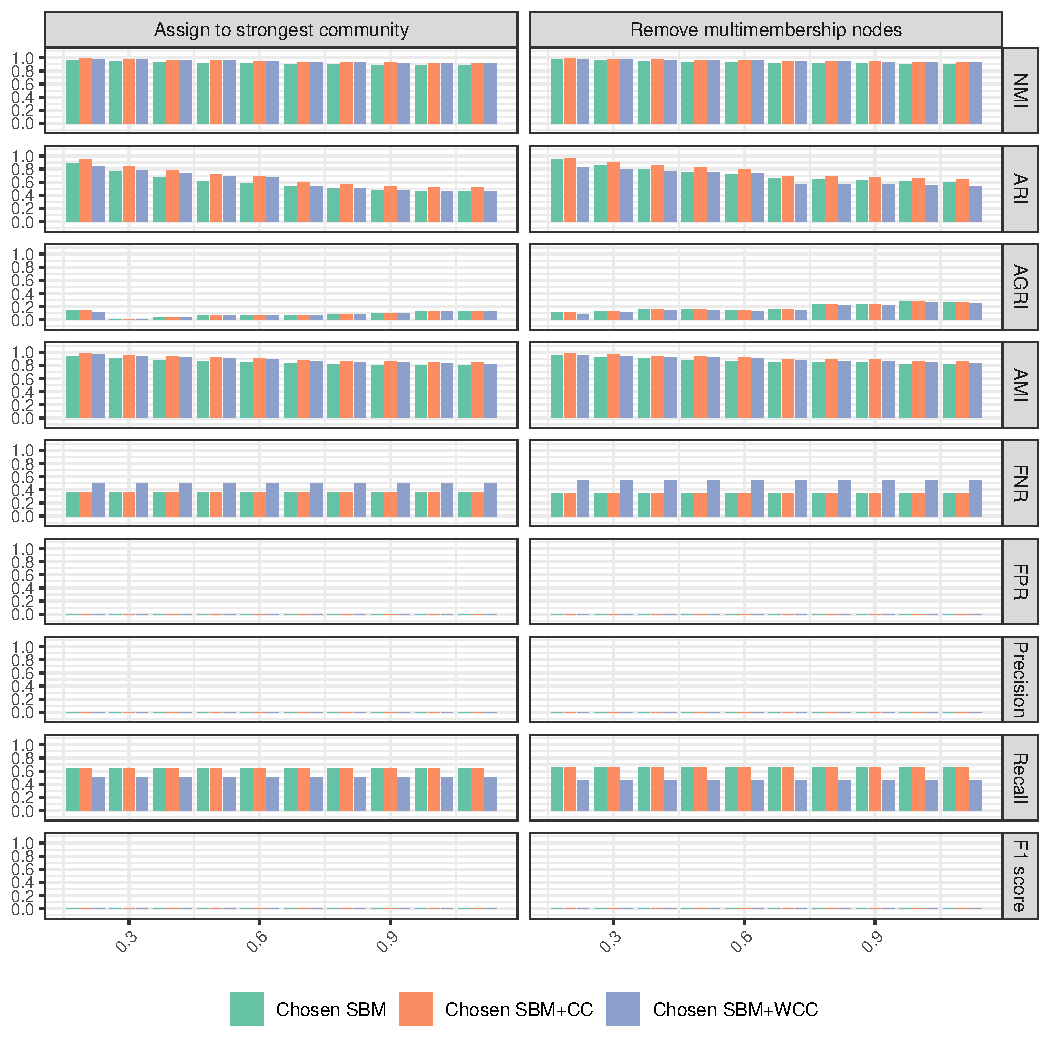
\includegraphics[width=0.9\textwidth]{figures/noise_livejournal_accuracy.pdf}
	\caption[]{\textbf{Various Clustering Accuracies for Varying Noise Levels on the Livejournal SNAP real-world network with ground-truth}}
	\label{fig:noise-livejournal-accuracy}
\end{figure}

\begin{figure}[!htpb]
	\centering
	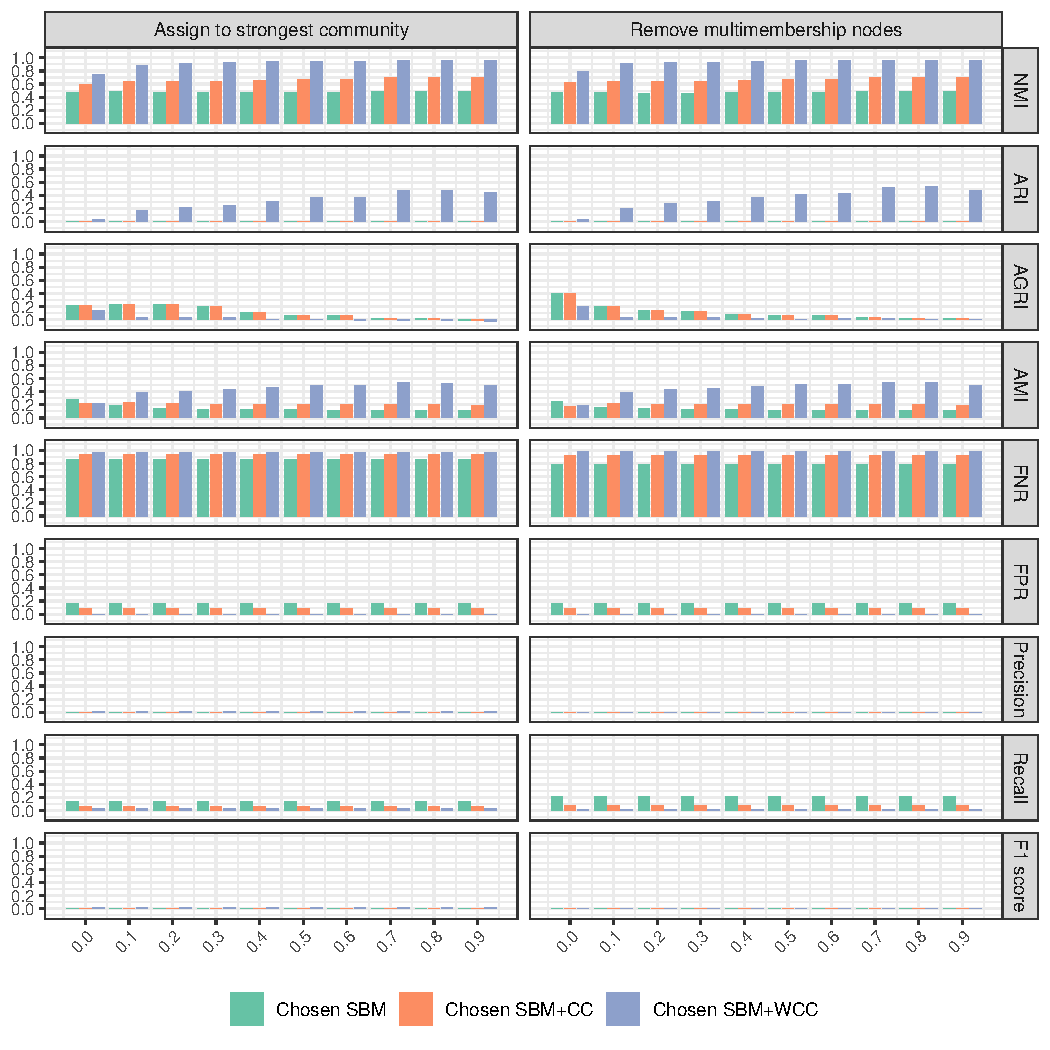
\includegraphics[width=0.9\textwidth]{figures/density_youtube_accuracy.pdf}
	\caption[]{\textbf{Various Clustering Accuracies for Varying Density Levels on the Youtube SNAP real-world network with ground-truth}}
	\label{fig:denisty-youtube-accuracy}
\end{figure}

\begin{figure}[!htpb]
	\centering
	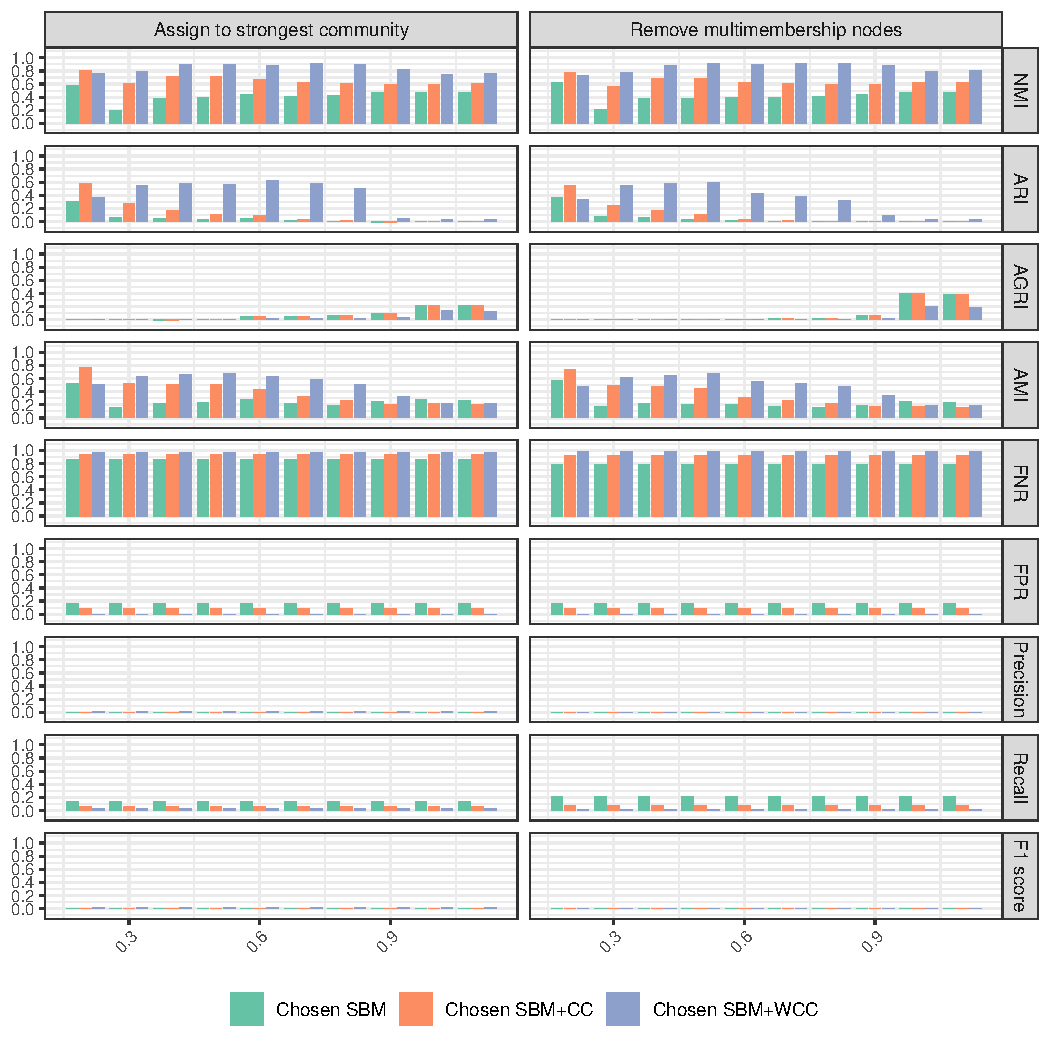
\includegraphics[width=0.9\textwidth]{figures/noise_youtube_accuracy.pdf}
	\caption[]{\textbf{Various Clustering Accuracies for Varying Noise Levels on the Youtube SNAP real-world network with ground-truth}}
	\label{fig:noise-youtube-accuracy}
\end{figure}


\begin{figure}[!htpb]
	\centering
	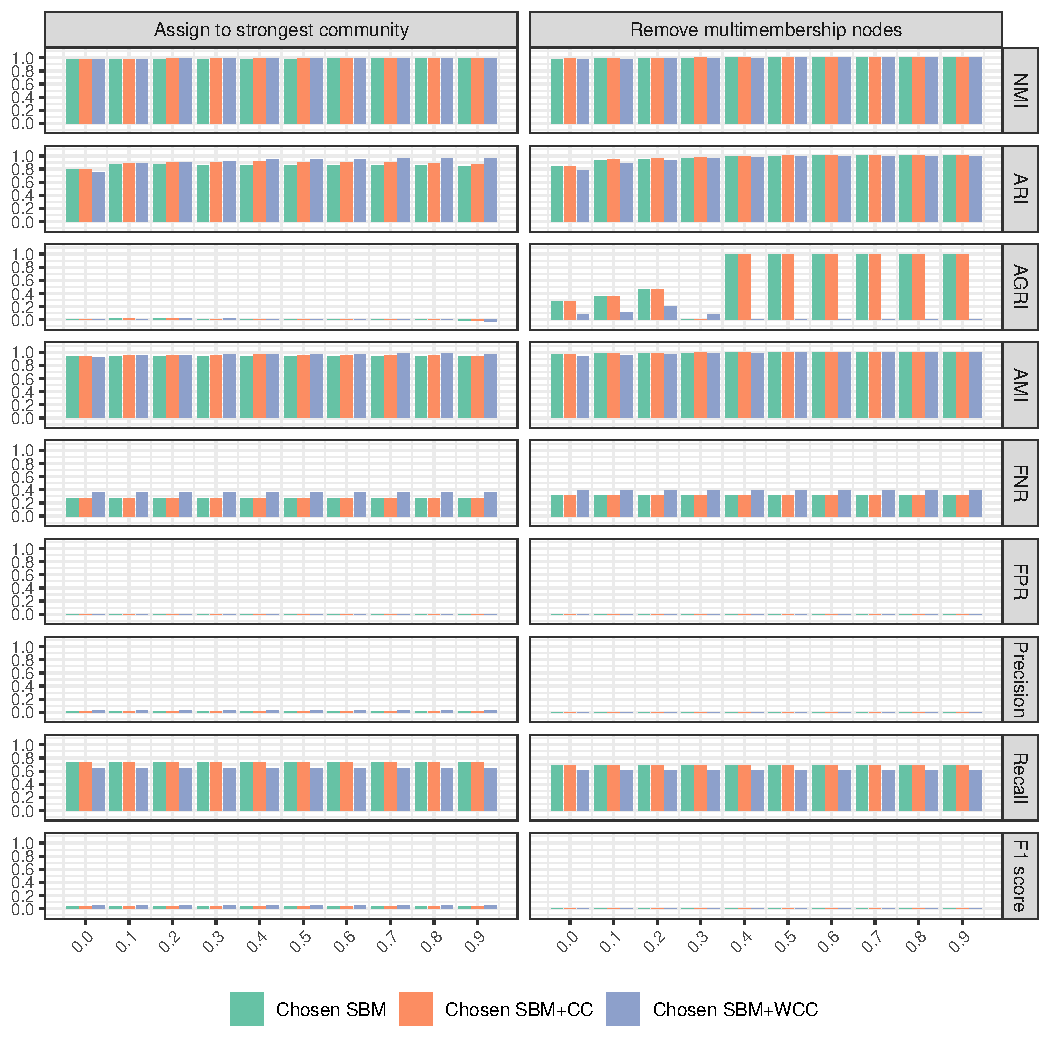
\includegraphics[width=0.9\textwidth]{figures/density_amazon_accuracy.pdf}
	\caption[]{\textbf{Various Clustering Accuracies for Varying Density Levels on the Amazon SNAP real-world network with ground-truth}}
	\label{fig:density-amazon-acuracy}
\end{figure}

\begin{figure}[!htpb]
	\centering
	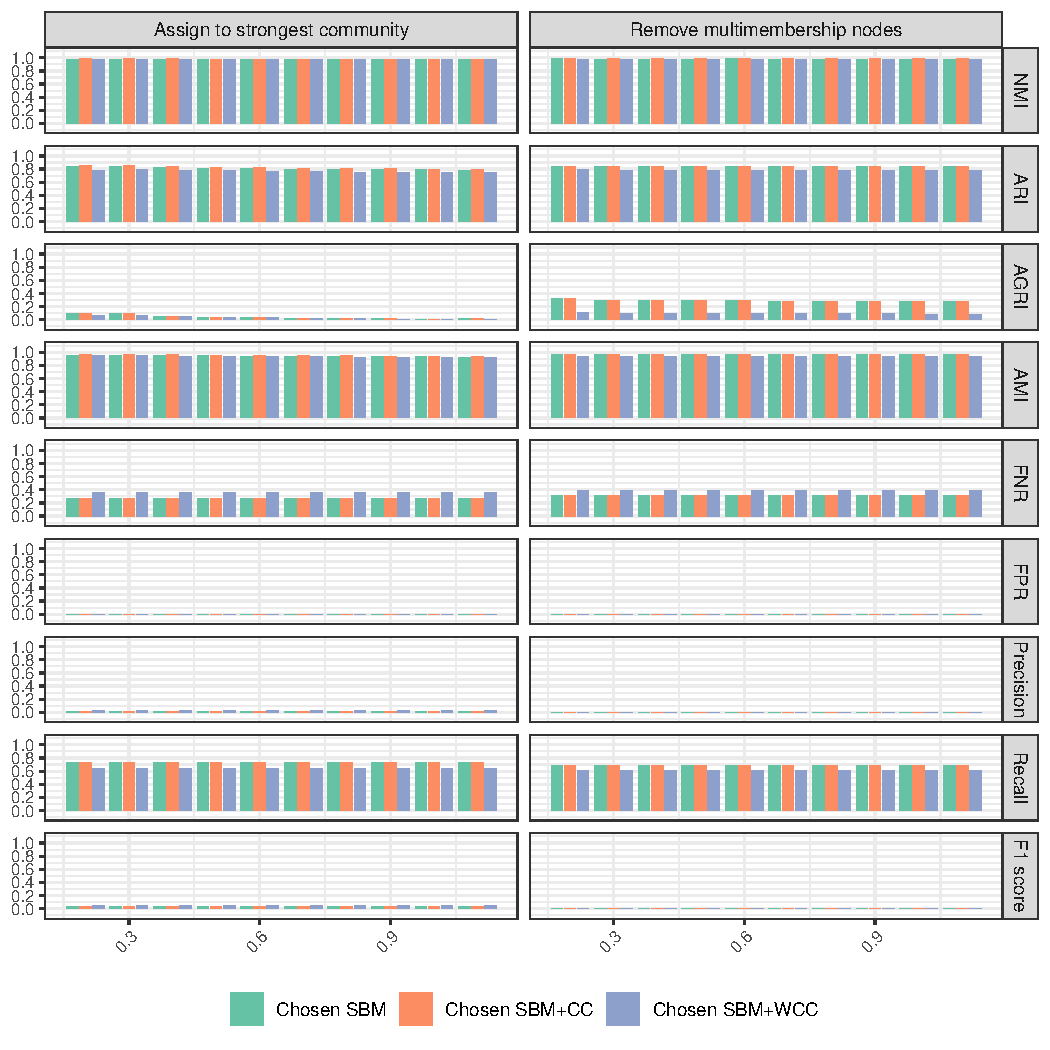
\includegraphics[width=0.9\textwidth]{figures/noise_amazon_accuracy.pdf}
	\caption[]{\textbf{Various Clustering Accuracies for Varying Noise Levels on the Amazon SNAP real-world network with ground-truth}}
	\label{fig:noise-amazon-acuracy}
\end{figure}

\begin{figure}[!htpb]
	\centering
	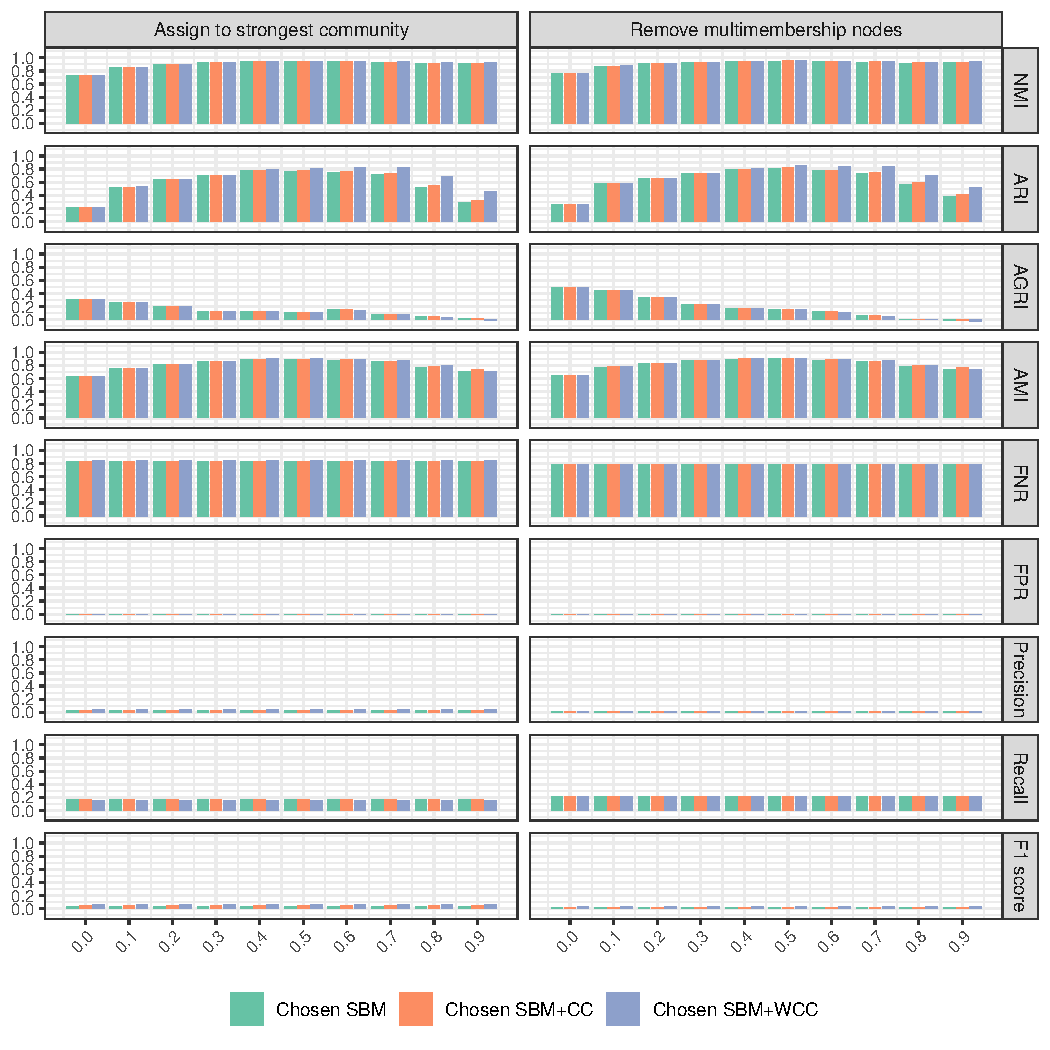
\includegraphics[width=0.9\textwidth]{figures/density_orkut_accuracy.pdf}
	\caption[]{\textbf{Various Clustering Accuracies for Varying Density Levels on the Orkut SNAP real-world network with ground-truth}}
	\label{fig:density-orkut-acuracy}
\end{figure}

\begin{figure}[!htpb]
	\centering
	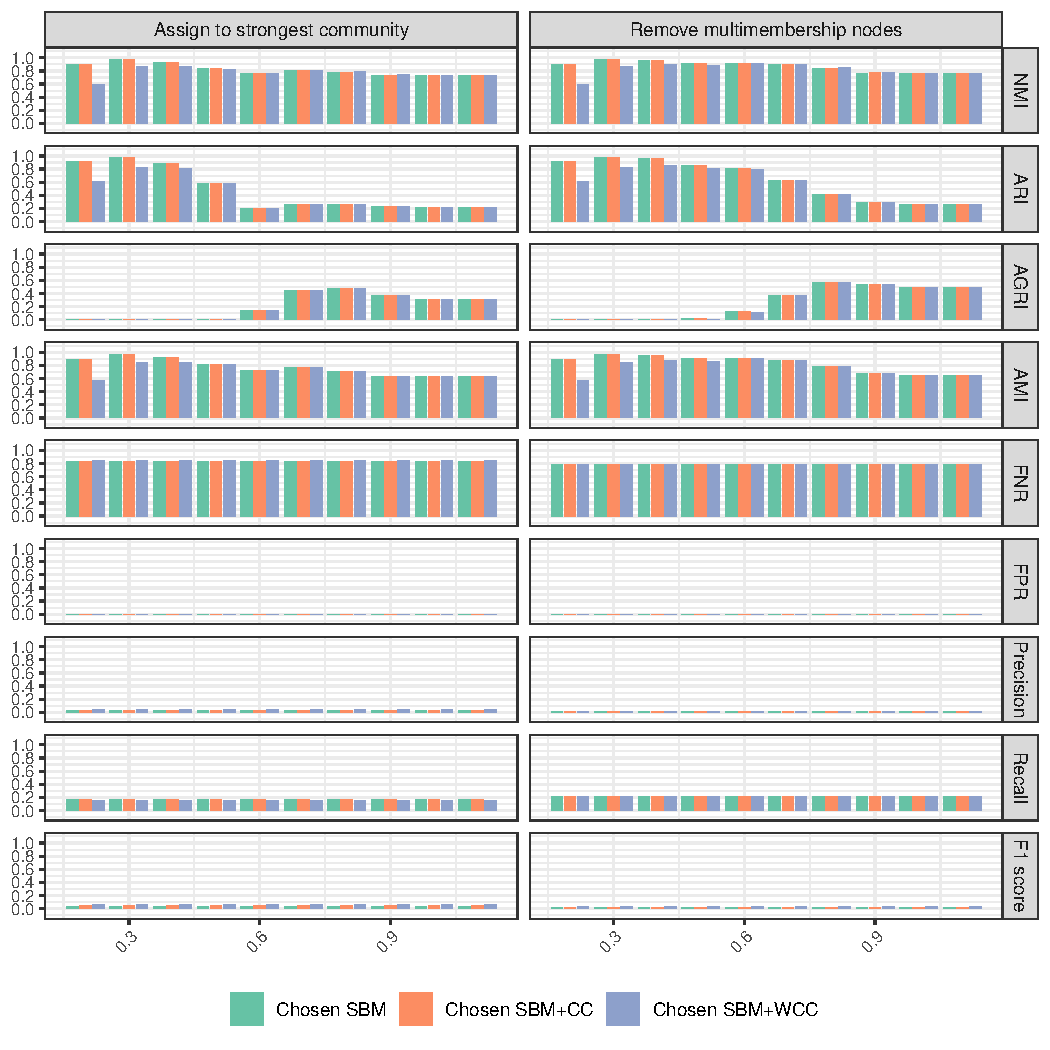
\includegraphics[width=0.9\textwidth]{figures/noise_orkut_accuracy.pdf}
	\caption[]{\textbf{Various Clustering Accuracies for Varying Noise Levels on the Orkut SNAP real-world network with ground-truth}}
	\label{fig:noise-orkut-acuracy}
\end{figure}

\clearpage


\newpage
\section{Results on SNAP networks: top 5000 clusters}


This next section has the results on SNAP networks, when we restrict attention to the top 5000 clusters.

\begin{table}[!htpb]
	\caption{\textbf{Cluster statistics of the top 5000 clusters of SNAP networks}}
	\begin{tabular}{lcrcrr}
		\hline
		dataset     & \multicolumn{2}{c}{\# edges per cluster} & \multicolumn{2}{c}{\# nodes per cluster} & \multicolumn{1}{c}{\# clusters (n \textgreater 100)}                                \\
		\hline

		            & min/median/max                           & mean                                     & min/median/max                                       & mean  & \multicolumn{1}{l}{} \\
		\hline
		\hline
		amazon      & 3/20.0/900                               & 39.8                                     & 3/8.0/328                                            & 13.5  & 31                   \\
		dblp        & 7/21.0/22699                             & 69.1                                     & 6/8.0/7556                                           & 22.4  & 54                   \\
		livejournal & 3/100.0/84155                            & 570.5                                    & 3/16.0/1441                                          & 27.8  & 145                  \\
		orkut       & 3/1590.5/156461                          & 3334.0                                   & 3/115.0/4785                                         & 215.7 & 2769                 \\
		youtube     & 1/3.0/9070                               & 30.4                                     & 2/4.0/2217                                           & 14.6  & 105                  \\
		\hline
	\end{tabular}


\end{table}

\clearpage

\begin{figure}[!htpb]
	\centering
	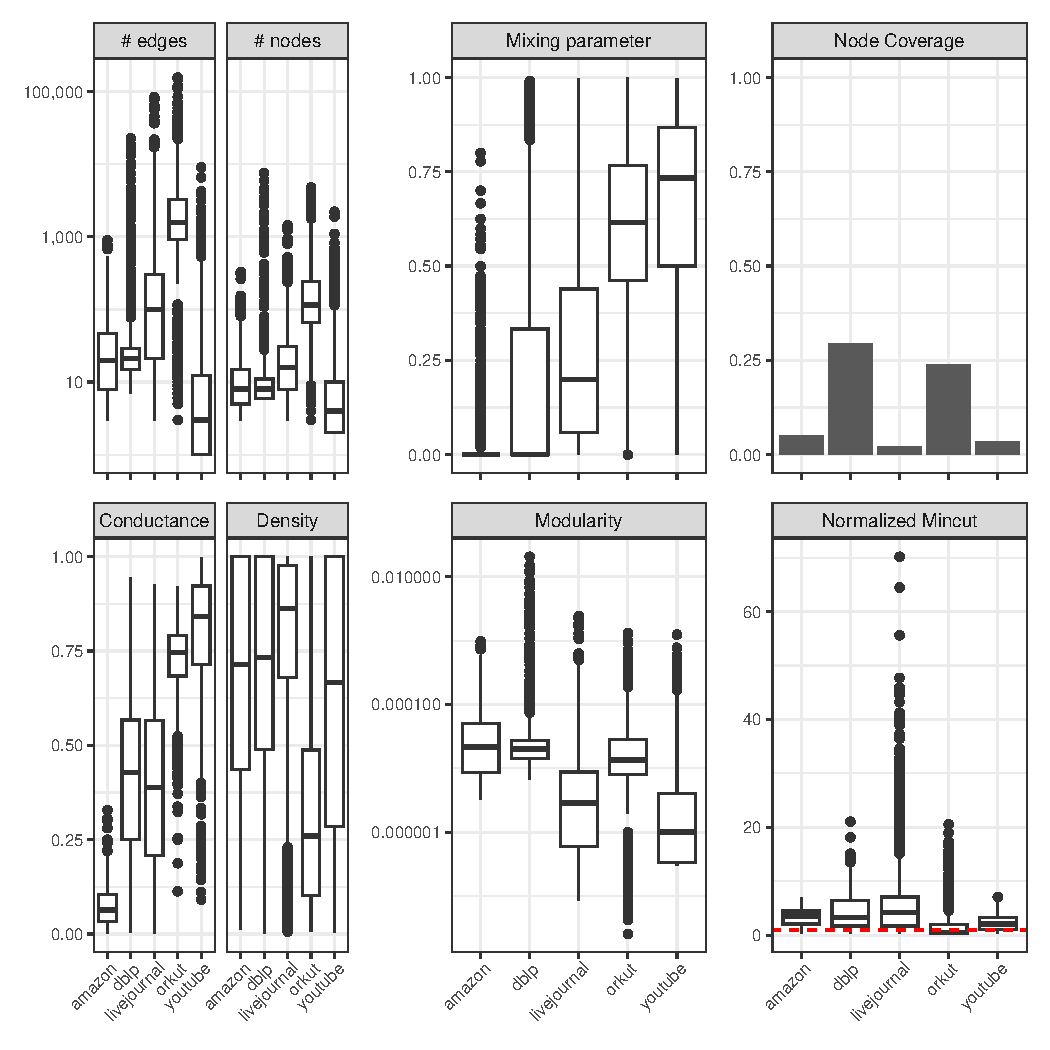
\includegraphics[width=0.9\textwidth]{figures/snap_groundtruth_top_5000_stats.pdf}
	\caption[]{\textbf{Network and Cluster Statistics for Top 5000 Ground-truth Clusters for the SNAP Collection} Top left: Number of edges and nodes in the network. Top center: Average of the mixing parameters across all nodes in the network and the node coverage of top-5000 ground-truth clusters. Top right: Distribution of edge and node counts over clusters of ground-truth. Bottom left: Distribution of conductance, density, and modularity over clusters of ground-truth. Bottom right: Distribution of normalized mincut sizes over clusters of ground-truth Red horizontal line indicates y=1, which is the threshold for well-connectedness.}
	\label{fig:XXX}
\end{figure}





\clearpage
\section{Formulas for cluster statistics}
Let $V$ be the set of all nodes in the network, $E$ be the set of all edges in the network, and $C$ be the mapping of node IDs to clusters IDs.

Assume that all edges are undirected and are only defined by two vertices $v_{i}$ and $v_{j}$, written as $e_{ij}$ so $e_{ij} = e_{ji}$.

The degree of a node $v_{i}$ is computed by $|\{e_{ij} :v_{i},v_{j} \in V \text{ and } i \neq j\}|$

All of the following calculations are done for a given cluster $c$ which is the set of nodes $\{v_{i} : C(v_{i}) = c\}$.

The sum of all node degrees in cluster $c$ is $k_{c} = \sum_{v_{i} \in c}{degree(v_{i})}$

Similarly, we can define $k_{c_{in}} = 2|\{e_{ij} : v_{i} \in c \text{ and } v_{j} \in c \text{ and } i \neq j\}|$ and $k_{c_{out}} = |\{e_{ij} : v_{i} \in c \text { and } v_{j} \notin c \text{ and } i \neq j\}|$

% $E_{cut}=\{e_{ij} : v_{i}\in c \text{ and } v_{j} \notin c \ \text{ and } i \neq j\}$





\vspace{.1in}
\textcolor{red}{Tandy's comments follow. }

\begin{itemize}

	\item It seems that $E_{cut}$ is exactly the same as $k_{c\_out}$. If so, just use one term and not the other.
	\item It looks like the denominator in Noise is exactly the same as $k_c$.
	\item Tandy;s comments about conductance are probably wrong. Ignore this.
	      'm looking right now at a definition for Conductance in another paper, see Section 2.1 in \url{http://snap.stanford.edu/class/cs224w-2018/reports/CS224W-2018-50.pdf}.    \textcolor{blue}{Min writes:I don't think by definition $k_{c} \leq |E|$ holds true since $k_{c}$ is upper-bounded by $2|E|$. We are double counting edges when summing the degree per node. I also put two subsections below that show that these two formulas end up giving the same numbers. I'm not confident that I didn't make any mistakes but intuitively I feel that $A(S)=k_{S}$ since both of them are counting the number of edges per node in $S$.}
	\item The definition of mixing parameter that you are using is not standard.  You are defining this term in order to have a way of talking about the ``mixing parameter of a cluster", but a different definition might be better. We can discuss.
	      But given the definition, it looks to be exactly the same as Noise.
	      Consider instead just writing down the distribution of individual mixing parameters of the nodes that are in the cluster.
	      That distribution can be then combined to
	      get the distribution of individual mixing
	      parameters for the clusters being considered.
\end{itemize}.



\subsection{Conductance}
A cluster $c$ defines a cut in which on one side of the cut is $c$ and the other side of the cut is $V \setminus c$. Therefore, the number of edges crossing the cut is simply $k_{c_{out}}$.


\begin{equation}
	Conductance(c) = \frac{k_{c_{out}}}{min(k_{c}, 2|E|-k_{c})}
\end{equation}

\subsubsection{Derivation of $A(S)$}
$A_{ij}$ is 1 if there is an edge between $v_{i}$ and $v_{j}$ and 0 otherwise since our input networks are considered unweighted.

\begin{align}
	A(S) & = \sum_{i \in S,j\in V}{A_{ij}}                                                                \\
	     & = \sum_{v_{i} \in S}{|{e_{ij} : v_{i} \in S \text{ and } v_{j} \in V \text { and } i \neq j}|} \\
	     & = \sum_{v_{i} \in S}{degree(v_{i})}
\end{align}

\subsubsection{Derivation of $A(\overline{S})$}
$A_{ij}$ is 1 if there is an edge between $v_{i}$ and $v_{j}$ and 0 otherwise since our input networks are considered unweighted.

\begin{align}
	A(\overline{S}) & = \sum_{i \in \overline{S},j\in V}{A_{ij}}                                                                           \\
	                & = \sum_{v_{i} \in \overline{S}}{|{e_{ij} : v_{i} \in \overline{S} \text{ and } v_{j} \in V \text { and } i \neq j}|} \\
	                & = \sum_{v_{i} \in \overline{S}}{degree(v_{i})}                                                                       \\
	                & = 2|E| - \sum_{v_{i} \in S}{degree(v_{i})}
\end{align}


\subsection{Noise}

\begin{equation}
	Noise = \frac{k_{c\_out}}{k_{c}}
\end{equation}

\subsection{Mixing parameter}
Quickly quoting LFR, ``2 Each node shares a fraction 1-$\mu$ of its links with the other nodes of its community and a fraction $\mu$ with the other nodes of the network; $\mu$ is the mixing parameter.''

The internal degree of a node $v_{i} \in c$ is $k_{v_{i}\_{in}}=|\{e_{ij} :v_{j} \in c \text{ and } i \neq j|$

The external degree of a node $v_{i} \in c$ is $k_{v_{i}\_{out}}=|\{e_{ij} :v_{j} \notin c |$

\begin{equation}
	MixingParameter(v_{i}) = \frac{k_{v_{i}\_out}}{k_{v_{i}\_in} + k_{v_{i}\_out}}
\end{equation}

\subsection{Density}
\begin{equation}
	Density=\frac{|\{e_{ij} : v_{i},v_{j} \in c \text{ and } i \neq j\}|}{{\binom{|N|}{2}}}
\end{equation}

\subsection{Normalized mincut size}
\begin{equation}
	NormalizedMincutSize=\frac{MincutSize}{\log_{10}{|c|}}
\end{equation}
% def conductance(self, graph):
%       num = self.get_border_edges(graph)
%       deg_sum = sum(graph.degree(v) for v in self.nodeset)
%       den = min(deg_sum, 2*graph.m() - deg_sum)
%       if den == 0:
%           # 1. singlenode cluster
%           # 2. entire graph is one cluster
%           # 3. cluster has no intracluster edges
%           return -42
%       return num/den

% \begin{figure}[!htpb]
% \centering
% \includegraphics[]{}
% \caption[]{\textbf{}}
% \label{fig:}
% \end{figure}

\section{Description Length Formulas}
\label{sbm-formulas}

\subsection{Microcanonical Non-Degree Corrected (SPC)}

Let $A$ be the adjacency matrix, $\vb{e}$ the edge matrix between blocks, and $\vb{b}$ the block assignments.
We optimize for minimum description length $\Sigma_{spc} = -\log_2P(A, \vb{e}, \vb{b}) = -\log_2 P(A \mid \vb{e}, \vb{b}) - \log_2 P(\vb{e} \mid \vb{b}) - \log_2 P(\vb{b})$, where
\begin{align}
	P(A \mid \vb{e}, \vb{b}) & = \frac{\prod_{r < s} e_{rs}! \prod_{r} e_{rr}!!}{\prod_r n_r^{e_r}} \frac{1}{\prod_{i < j} A_{ij}! \prod_{i} A_{ii}!!} \\
	P(\vb{e} \mid \vb{b})    & = \left( \binom{K(K+1)/2}{M} \right)^{-1}                                                                               \\
	P(\vb{b})                & = \frac{\prod_r n_r!}{N!} \binom{N - 1}{M - 1}^{-1} \frac{1}{N}
\end{align}
where $N$ is the total number of nodes, $M$ the total number of edges, $K$ the number of blocks, $\left( \binom{n}{k} \right) = \binom{n + k - 1}{k}$, and $(2n)!! = 2^n n!$.
See equations (23-25) of ~\cite{peixoto17-01}, or (13-15) of ~\cite{funke19-04}.

In graph-tool, this corresponds to the parameters
\begin{verbatim}
    BlockState(g, b, deg_corr=False).entropy()
\end{verbatim}

\subsection{Microcanonical Degree Corrected (DCPU)}

Let $A$ be the adjacency matrix, $\vb{e}$ the edge matrix between blocks, $\vb{k}$ the degree vector (per node), and $\vb{b}$ the block assignments (per node).
We optimize for minimum description length $\Sigma_{dpcu} = -\log_2P(A, \vb{k}, \vb{e}, \vb{b}) = -\log_2P(A \mid \vb{k}, \vb{e}, \vb{b}) - \log_2 P(\vb{k} \mid \vb{e}, \vb{b}) - \log_2 P(\vb{e} \mid \vb{b}) - \log_2 P(\vb{b}) $, where
\begin{align}
	P(A \mid \vb{k}, \vb{e}, \vb{b}) & = \frac{ \prod_i k_i! \prod_{r < s} e_{rs}! \prod_{r} e_{rr}!!} {\prod_{i < j} A_{ij}! \prod_i A_{ii}!! \prod_r e_r!}                                      \\
	P(\vb{k} \mid \vb{e}, \vb{b})    & = \prod_r \left( \binom{n_r}{e_r} \right)^{-1}                                                                                                             \\
	P(\vb{e} \mid \vb{b})            & = \prod_{l=1}^{L} \prod_{r < s} \left( \binom{n_r^l n_s^l}{e_{rs}^{l+1}} \right)^{-1} \prod_r \left( \binom{ n_r^l (n_r^l + 1) / 2 }{e_{rr}^{l+1} }\right) \\
	P(\vb{b})                        & = \prod_{l=1}^L \frac{\prod_r n_r^l!}{K^{l-1}!} \binom{ K^{l-1} - 1}{K^l - 1}^{-1} \frac{1}{K^{l-1}}
\end{align}
where $N$ is the total number of nodes, $M$ the total number of edges, $K$ the number of blocks, $\left( \binom{n}{k} \right) = \binom{n + k - 1}{k}$, and $(2n)!! = 2^n n!$.
See equations (1-3), (26) in ~\cite{peixoto17-01}, or (16-18) of ~\cite{funke19-04}.

In graph-tool, this corresponds to the parameters
\begin{verbatim}
    BlockState(g, b, deg_corr=False, entropy_args={ degree_dl_kind = "uniform" }).entropy()
\end{verbatim}

\subsection{Microcanonical Degree Corrected (DCPUH)}

Let $A$ be the adjacency matrix, $\vb{e}$ the edge matrix between blocks, $\vb{k}$ the degree vector (per node), and $\vb{b}$ the block assignments (per node).
We optimize for minimum description length $\Sigma_{dpcuh} = -\log_2P(A, \vb{k}, \vb{e}, \vb{b}) = -\log_2P(A \mid \vb{k}, \vb{e}, \vb{b}) - \log_2 P(\vb{k} \mid \vb{e}, \vb{b}) - \log_2 P(\vb{e} \mid \vb{b}) - \log_2 P(\vb{b}) $, where
\begin{align}
	P(A \mid \vb{k}, \vb{e}, \vb{b}) & = \frac{ \prod_i k_i! \prod_{r < s} e_{rs}! \prod_{r} e_{rr}!!} {\prod_{i < j} A_{ij}! \prod_i A_{ii}!! \prod_r e_r!}                                      \\
	P(\vb{k} \mid \vb{e}, \vb{b})    & = \prod_r \frac{\prod_k N_k^r!}{n_r!} q(e_r, n_r)^{-1}                                                                                                     \\
	P(\vb{e} \mid \vb{b})            & = \prod_{l=1}^{L} \prod_{r < s} \left( \binom{n_r^l n_s^l}{e_{rs}^{l+1}} \right)^{-1} \prod_r \left( \binom{ n_r^l (n_r^l + 1) / 2 }{e_{rr}^{l+1} }\right) \\
	P(\vb{b})                        & = \prod_{l=1}^L \frac{\prod_r n_r^l!}{K^{l-1}!} \binom{ K^{l-1} - 1}{K^l - 1}^{-1} \frac{1}{K^{l-1}}
\end{align}
where $N_k^r$ denotes the number of nodes with degree $k$ in group $r$ and $q(m, n)$ the number of partitions of $m$ into $n$ parts.
That is,
\begin{equation}
	q(m, n) =
	\begin{cases}
		1                         & m = n = 0        \\
		0                         & n = 0, m > 0     \\
		q(m, m)                   & n > m            \\
		q(m, n - 1) + q(m - n, n) & \text{otherwise}
	\end{cases}
\end{equation}
See equations (1-3), (27-30) in ~\cite{peixoto17-01}, or (16-18) of ~\cite{funke19-04}.

In graph-tool, this corresponds to the parameters
\begin{verbatim}
    BlockState(g, b, deg_corr=False, entropy_args={ degree_dl_kind = "distributed" }).entropy()
\end{verbatim}

\subsection{Microcanonical Non-Degree Corrected (HSPC)}

Let $A$ be the adjacency matrix, $\vb{e}$ the edge matrix between blocks, and $\vb{b}$ the block assignments.
We optimize for minimum description length $\Sigma_{hspc} = -\log_2P(A, \vb{e}, \vb{b}) = -\log_2 P(A \mid \vb{e}, \vb{b}) - \log_2 P(\vb{e} \mid \vb{b}) - \log_2 P(\vb{b})$, where
\begin{align}
	P(A \mid \vb{e}, \vb{b}) & = \frac{\prod_{r < s} e_{rs}! \prod_{r} e_{rr}!!}{\prod_r n_r^{e_r}} \frac{1}{\prod_{i < j} A_{ij}! \prod_{i} A_{ii}!!}                                    \\
	P(\vb{e} \mid \vb{b})    & = \prod_{l=1}^{L} \prod_{r < s} \left( \binom{n_r^l n_s^l}{e_{rs}^{l+1}} \right)^{-1} \prod_r \left( \binom{ n_r^l (n_r^l + 1) / 2 }{e_{rr}^{l+1} }\right) \\
	P(\vb{b})                & = \prod_{l=1}^L \frac{\prod_r n_r^l!}{K^{l-1}!} \binom{ K^{l-1} - 1}{K^l - 1}^{-1} \frac{1}{K^{l-1}}
\end{align}
where $N$ is the total number of nodes, $M$ the total number of edges, $K$ the number of blocks, $\left( \binom{n}{k} \right) = \binom{n + k - 1}{k}$, and $(2n)!! = 2^n n!$.
See equations (23-25), (41-42) of ~\cite{peixoto17-01}, or (13-15), (19-20) of ~\cite{funke19-04}.

In graph-tool, this corresponds to the parameters
\begin{verbatim}
    NestedBlockState(g, b, deg_corr=False).entropy()
\end{verbatim}

\subsection{Microcanonical Degree Corrected (HDCPU)}

Let $A$ be the adjacency matrix, $\vb{e}$ the edge matrix between blocks, $\vb{k}$ the degree vector (per node), and $\vb{b}$ the block assignments (per node).
We optimize for minimum description length $\Sigma_{hdpcu} = -\log_2P(A, \vb{k}, \vb{e}, \vb{b}) = -\log_2P(A \mid \vb{k}, \vb{e}, \vb{b}) - \log_2 P(\vb{k} \mid \vb{e}, \vb{b}) - \log_2 P(\vb{e} \mid \vb{b}) - \log_2 P(\vb{b}) $, where
\begin{align}
	P(A \mid \vb{k}, \vb{e}, \vb{b}) & = \frac{ \prod_i k_i! \prod_{r < s} e_{rs}! \prod_{r} e_{rr}!!} {\prod_{i < j} A_{ij}! \prod_i A_{ii}!! \prod_r e_r!}                                      \\
	P(\vb{k} \mid \vb{e}, \vb{b})    & = \prod_r \left( \binom{n_r}{e_r} \right)^{-1}                                                                                                             \\
	P(\vb{e} \mid \vb{b})            & = \prod_{l=1}^{L} \prod_{r < s} \left( \binom{n_r^l n_s^l}{e_{rs}^{l+1}} \right)^{-1} \prod_r \left( \binom{ n_r^l (n_r^l + 1) / 2 }{e_{rr}^{l+1} }\right) \\
	P(\vb{b})                        & = \prod_{l=1}^L \frac{\prod_r n_r^l!}{K^{l-1}!} \binom{ K^{l-1} - 1}{K^l - 1}^{-1} \frac{1}{K^{l-1}}
\end{align}
where $N$ is the total number of nodes, $M$ the total number of edges, $K$ the number of blocks, $\left( \binom{n}{k} \right) = \binom{n + k - 1}{k}$, and $(2n)!! = 2^n n!$.
See equations (1-3), (26), (41-42) in ~\cite{peixoto17-01}, or (16-18) of ~\cite{funke19-04}.

In graph-tool, this corresponds to the parameters
\begin{verbatim}
    NestedBlockState(g, b, deg_corr=False, entropy_args={ degree_dl_kind = "uniform" }).entropy()
\end{verbatim}

\subsection{Microcanonical Degree Corrected (HDCPUH)}

Let $A$ be the adjacency matrix, $\vb{e}$ the edge matrix between blocks, $\vb{k}$ the degree vector (per node), and $\vb{b}$ the block assignments (per node).
We optimize for minimum description length $\Sigma_{hdpcuh} = -\log_2P(A, \vb{k}, \vb{e}, \vb{b}) = -\log_2P(A \mid \vb{k}, \vb{e}, \vb{b}) - \log_2 P(\vb{k} \mid \vb{e}, \vb{b}) - \log_2 P(\vb{e} \mid \vb{b}) - \log_2 P(\vb{b}) $, where
\begin{align}
	P(A \mid \vb{k}, \vb{e}, \vb{b}) & = \frac{ \prod_i k_i! \prod_{r < s} e_{rs}! \prod_{r} e_{rr}!!} {\prod_{i < j} A_{ij}! \prod_i A_{ii}!! \prod_r e_r!}                                      \\
	P(\vb{k} \mid \vb{e}, \vb{b})    & = \prod_r \frac{\prod_k N_k^r!}{n_r!} q(e_r, n_r)^{-1}                                                                                                     \\
	P(\vb{e} \mid \vb{b})            & = \prod_{l=1}^{L} \prod_{r < s} \left( \binom{n_r^l n_s^l}{e_{rs}^{l+1}} \right)^{-1} \prod_r \left( \binom{ n_r^l (n_r^l + 1) / 2 }{e_{rr}^{l+1} }\right) \\
	P(\vb{b})                        & = \prod_{l=1}^L \frac{\prod_r n_r^l!}{K^{l-1}!} \binom{ K^{l-1} - 1}{K^l - 1}^{-1} \frac{1}{K^{l-1}}
\end{align}
where $N_k^r$ denotes the number of nodes with degree $k$ in group $r$ and $q(m, n)$ the number of partitions of $m$ into $n$ parts.
That is,
\begin{equation}
	q(m, n) =
	\begin{cases}
		1                         & m = n = 0        \\
		0                         & n = 0, m > 0     \\
		q(m, m)                   & n > m            \\
		q(m, n - 1) + q(m - n, n) & \text{otherwise}
	\end{cases}
\end{equation}
See equations (1-3), (27-30), (42) in ~\cite{peixoto17-01}, or (16-18), (19-20) of ~\cite{funke19-04}.

In graph-tool, this corresponds to the parameters
\begin{verbatim}
    NestedBlockState(g, b, deg_corr=False, entropy_args={degree_dl_kind="distributed"}).entropy()
\end{verbatim}

\clearpage
\bibliography{refs}
\bibliographystyle{ACM-Reference-Format}

\end{document}
